
\documentclass[12pt,singleside,a4paper]{article}



\usepackage[utf8]{inputenc}
\usepackage{mwe}
\usepackage{graphicx}
\usepackage{epsfig}
\usepackage{cite}
\usepackage{geometry}
\usepackage{float}
\usepackage{subfig}
\usepackage{comment}
\usepackage{listings}
\usepackage{minted}
\usepackage{hyperref}
\usepackage[usenames,dvipsnames]{xcolor}


\definecolor{vgreen}{RGB}{104,180,104}
\definecolor{vblue}{RGB}{49,49,255}
\definecolor{vorange}{RGB}{255,143,102}


\lstdefinestyle{verilog-style}
{
    language=Verilog,
    frame=single,
    linewidth=18.5cm,
    basicstyle=\small\ttfamily,
    keywordstyle=\color{vblue},
    identifierstyle=\color{black},
    commentstyle=\color{vgreen},
    moredelim=*[s][\colorIndex]{[}{]},
    literate=*{:}{:}1
}

%%%%%%%%%%%%%%%%%vhdl%%%%%%%%%%%%%%%%%%%%

\lstdefinelanguage{VHDL}{
   morekeywords=[1]{
     LIBRARY,USE,ENTITY,IS,PORT,IN,OUT,END,ARCHITECTURE,OF,
     BEGIN,DOWNTO,ALL,WAIT,FOR,OTHERS,SIGNAL,PROCESS,     library,use,entity,is,port,in,out,end,architecture,of,
     begin,downto,all,wait,for,others,signal,proces, COMPONENT, component, process, variable, while, next, for, when
   },
   morekeywords=[2]{
     STD_LOGIC_VECTOR,STD_LOGIC,IEEE,STD_LOGIC_1164,
     NUMERIC_STD,STD_LOGIC_ARITH,STD_LOGIC_UNSIGNED,std_logic_vector,AND,OR,NOT,NAND,NOR,XOR,
     std_logic,     std_logic_vector,std_logic,ieee,std_logic_1164,
     numeric_std,std_logic_arith,std_logic_unsigned,std_logic_vector,and,or,not,nand,nor,xor,
     std_logic, readline, read
   },
   morecomment=[l]--
}
\colorlet{keyword}{blue!100!black!80}
\colorlet{STD}{Lavender}
\colorlet{comment}{green!80!black!90}
\lstdefinestyle{vhdl}{
   language     = VHDL,
   basicstyle   = \footnotesize \ttfamily,
   keywordstyle = [1]\color{keyword}\bfseries,
   keywordstyle = [2]\color{STD}\bfseries,
   commentstyle = \color{comment}
}
%%%%%%%%%%%%%%%%%%%%%%%%%%%%%%%%%%%%%%%%%%%%%%%%%%%

\geometry{left=20mm,right=20mm,top=20mm,bottom=40mm}


\begin{document} 
\begin{titlepage}
	\centering
    \textsc{\LARGE 8 Bit Arithmetic Logic Unit}\\[2.0 cm]
\begin{figure}[!htb]
\centering
  
\includegraphics[width=3cm,keepaspectratio]{logo.png}\textbf{ }\textbf{  }
  
\includegraphics[width=3cm,keepaspectratio]{download.png}\textbf{  }
  
\includegraphics[width=3cm,keepaspectratio]{modelsim-logo.jpg}
\end{figure}	\\[2cm]\
	\begin{minipage}{0.4\textwidth}
		\begin{flushleft} \large
			\emph{Mentors}\\
			Prasad T\\
            Aditya Gudla\\
            Simranjeet Singh \
			\end{flushleft}
			\end{minipage}~
			\begin{minipage}{0.4\textwidth}
            
			\begin{flushright} \large
			\emph{Interns} \\
			Ajay Chaudhari\\
            Chethan T Bhat\\
            Ritvik Tiwari \\
            Karthik A Shet \\
		\end{flushright}
	\end{minipage}\\[2 cm]
\end{titlepage}
\pagenumbering{arabic}

\newpage


\tableofcontents

\newpage
\section{Introduction}
An arithmetic logic unit (ALU) is a digital circuit used to perform arithmetic and logic operations. It represents the fundamental building block of the central processing unit (CPU) of a computer. Modern CPUs contain very powerful and complex ALUs. In addition to ALUs, modern CPUs contain a control unit (CU).

Most of the operations of a CPU are performed by one or more ALUs, which load data from input registers. A register is a small amount of storage available as part of a CPU. The control unit tells the ALU what operation to perform on that data, and the ALU stores the result in an output register. The control unit moves the data between these registers, the ALU, and memory. 

\subsection{Problem Statement.}
 To Design an 8-bit ALU which performs different set of Arithmetic and logical operations based on the select input 's'.It includes writing, compiling and simulating Verilog code in Quartus II and  ModelSim respectively.

\newline



\subsection{Block Diagram 8-bit ALU.}
\begin{figure}[H]
    \centering
    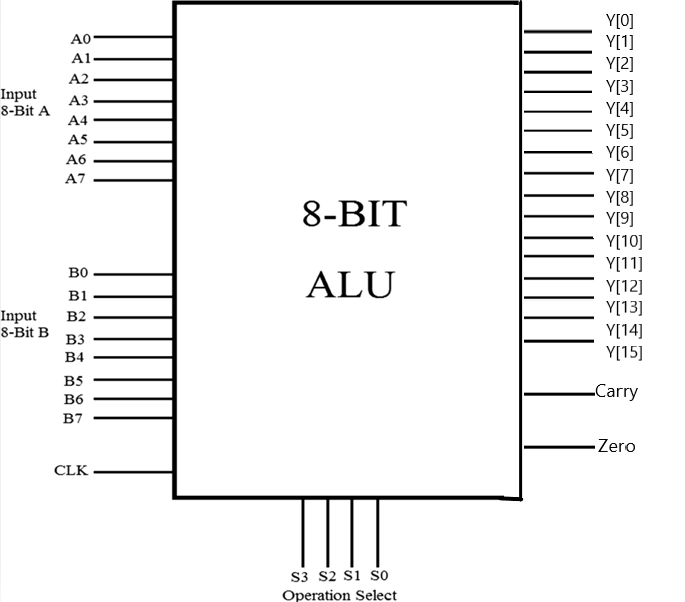
\includegraphics[scale=0.8]{NEWALUBLOCK.png}
    \caption{Block Diagram of 8bit ALU}
\end{figure}
\newpage
\subsection{Implementation Table of 8-bit ALU.}
The below table indicates the Arithmetic and Logical operations performed based on the select input 's' and also the output 'y' obtained for for the given set of input 'a' and 'b'.
\vspace{8mm}
The Arithmetic opertaions that are performed here are:
\begin{itemize}
 
    \item Addition
    \item Subtraction
    \item Multiplication
    \item Division
    \item Increment
    \item Decrement
    
\end{itemize}
Some of the Logical operations performed here are:
\begin{itemize}
    \item Bitwise AND \& NAND
    \item Bitwise OR \& NOR
    \item Bitwise NOR \& XNOR
    \item Shift Right \& Shift Left
    \item Rotate Right \& Rotate Left
\end{itemize}
\begin{center}
\begin{tabular}{ |p{1cm}|p{3cm}|p{2cm}|p{2cm}|p{4cm}|p{1cm}|p{1cm}| } \hline
 \multicolumn{7}{|c|}{Implementation Table of 8-bit ALU}   \\ \hline \hline
    s      &    operation        &  a           &  b           &   y             &   carry &   zero      \\ \hline
    0000   &    Addition         &   11101110   &   11101110   &   00000000 11011100      &    1      &  0          \\ \hline
    0001   &    Subtraction      &   11101110   &   11101110   &   00000000 00000000      &    0      &  1         \\\hline
    0010   &    Increment        &   11101110   &   11101110   &   00000000 11101111      &    0      &  0         \\\hline
    0011   &    Decrement        &   11101110   &   11101110   &   00000000 11101101      &    0      &  0          \\\hline
    0100   &    Multiplication   &   11101110   &   11101110   &   11011101 01000100‬     &    0      &  0          \\\hline
    0101   &    Division         &   11101110   &   11101110   &   00000000 00000001      &    0      &  0          \\\hline
     
    
    0110   &    Bitwise AND      &   11101110   &   11101110   &   00000000 11101110      &    0      &  0          \\\hline
    0111   &    Bitwise OR       &   11101110   &   11101110   &   00000000 11101110      &    0      &  0          \\\hline
    1000   &    Bitwise XOR      &   11101110   &   11101110   &   00000000 00000000      &    0      &  1         \\\hline
    1001   &   Bitwise NAND     &   11101110   &   11101110   &   00000000 00010001      &    0      &  0          \\\hline
    1010   &   Bitwise NOR       &   11101110   &   11101110   &   00000000 00010001      &    0      &  0          \\\hline
    1011   &    Bitwise XNOR     &   11101110   &   11101110   &   00000000 11111111      &    0      &  0          \\\hline
    1100   &    Shift Left       &   11101110   &   11101110   &   00000000 11011100      &    1      &  0         \\\hline
    1101   &    Shift Right      &   11101110   &   11101110   &   00000000 01110111      &    0      &  0         \\\hline
    1110   &    Rotate Right     &   11101110   &   11101110   &  00000000  01110111      &    0      &  0          \\\hline
    1111   &    Rotate Left      &   11101110   &   11101110   &   00000000 11011101      &    0      &  0          \\\hline
\end{tabular} 
\captionof{table}{Implementation Table of 8-bit ALU}
\end{center}

\newpage
\section{Verilog HDL Codes for 8-bit ALU}


\subsection{RTL Description}
\begin{lstlisting}[style=verilog-style]
  //Verilog Design for a 8-bit ALU.
  /*This design will Perform Arithmetic and Logical operations 
  based on the select input */

  //Define module.
  module  ALU(
	input [7:0]a,b,
	input [3:0]s,      //Define Inputs a,b and select line input s
	input en,clk,		    //Define clock and enable signal
	output [15:0] y,     //Define 16 bit ALU output
	output carry, zero  //Define Flag output
	);
	
  reg [7:0]a_in;	    //Local registers for input 'a'.
  reg [7:0]b_in;	    //Local registers for input 'b'.
  reg [1:0]flags;	    
  /*Local register to store carry bit in flags[0] &
  zero flag bit in flags[1]*/
  reg [15:0] out_y;   //Local register to store 16 bit output 'y'.


 always @(posedge clk, negedge en)
 begin
    if(en==1)		//if en=1, reset all outputs
    begin
        a_in <= 0;
        b_in <= 0;
        y <= 0;
        carry <= 0;
        zero <= 0;
    end
    else
    begin
        a_in <= a;   //if en=1, latch all output flit flops
        b_in <= b;
        y <= out_y;
        carry <= flags[0];
        zero <= flags[1];
    end
 end
 

 \end{lstlisting}
 \newpage
 \begin{lstlisting}[style=verilog-style]
 always @ (a_in,b_in,s)  
 begin
    flags = 2'b00;  //set flags to zero
    case(s)
        4'd0:
        begin
            out_y={8'd0,(a_in + b_in)}; //addition
            flags[0]=out_y[8];  //carry is set if generated.
        end	
        4'd1:
        begin
            out_y={8'd0,(a_in - b_in)};	 //Subtraction
            flags[0]=out_y[8];  //carry is set if Borrow is taken.
        end 
        4'd2:
        begin 
            out_y={8'd0,(a_in + 1'b1)};	 //Increment
            flags[0]=out_y[8];   //carry is set if generated.
        end
        4'd3:begin
            out_y={8'd0,(a_in - 1'b1)};	 //Decrement
            flags[0]=out_y[8]; //carry is set if Borrow is taken.
        end
        4'd4:out_y=(a_in * b_in);          //Multiplication.
        4'd5:out_y=(a_in / b_in);		   //Division
        4'd6:out_y={8'd0,(a_in & b_in)};   //Bitwise AND
        4'd7:out_y={8'd0,(a_in | b_in)};   //Bitwise OR
        4'd8:out_y={8'd0,(a_in ^ b_in)};   //Bitwise XOR
        4'd9:out_y={8'd0,~(a_in & b_in)};  //Bitwise NAND
        4'd10:out_y={8'd0,~(a_in | b_in)}; //Bitwise NOR
        4'd11:out_y={8'd0,~(a_in ^ b_in)}; //Bitwise XNOR
        4'd12:
        begin
            flags[0] = a_in[7];         //Update carry flag
            out_y={8'd0,(a_in<<1)};     //Shift Left
        end	
        4'd13:begin
            flags[0] = a_in[0];       //Update carry flag
            out_y={8'd0,(a_in>>1)};   //Shift Right
        end
        4'd14: out_y ={8'd0,a_in[0],a_in[7:1]}; //right rotate
        4'd15: out_y={8'd0,a_in[6:0],a_in[7]};   //left rotate
        default: out_y=16'd0;
	endcase
    if(out_y == 0)
        flags[1] = 1;    //set zero flag if output is zero
 end                       //End of case structure. 
endmodule					// End of module.
\end{lstlisting}
\newpage

\subsection{Testbench for 8-bit ALU.}
\begin{lstlisting}[style=verilog-style]

//Verilog code for TestBench of 8-bit ALU

//Define module
module tb_ALU;
reg [7:0]a; reg [7:0]b; reg [3:0]s;         // Define I/O ports
reg clk; reg en; 
wire [15:0]y;
wire carry;
wire zero;


//Map all the I/O ports with DUT.
ALU uut(.a(a),.b(b),.s(s),.en(en),.clk(clk),.y(y),.carry(carry),.zero(zero));


//Initialise Input pins with 0
initial begin
	a = 0;
	b = 0;
	s = 0;
	en=1;
	clk = 0;
end

always
begin clk = ~clk;#5; end      //Generate a clock of period 10 units

initial begin
#50;
	a = 8'b11101110;    //	Initialise 8bit input value for a & b.
	b = 8'b11101110;#29;

// Initialise 's' value to perform different operations.	
	s = 4'b0001;#30;   
	s = 4'b0010;#30;
	en=0
	s = 4'b0001;#30;   
	s = 4'b0010;#30;
	s = 4'b0011;#30;
	s = 4'b0100;#30;
	s = 4'b0101;#30;
	s = 4'b0110;#30;
	s = 4'b0111;#30;
	s = 4'b1000;#30;
	s = 4'b1001;#30;
\end{lstlisting}
\newpage
\begin{lstlisting}[style=verilog-style]
	s = 4'b1010;#30;
	s = 4'b1011;#30;
	s = 4'b1100;#30;
	s = 4'b1101;#30;
	s = 4'b1110;#30;
	s = 4'b1111;#30;
end                           // End of initial block
endmodule					      // End of module.

	
	
	
\end{lstlisting}

\newpage
\section{VHDL Codes for 8-bit ALU}
You can perform the same experiment using \textbf{VHDL} language.
Please refer the codes given below.
\textbf{Code for 8-bit ALU}
\subsection{RTL Description}
\begin{lstlisting}[style=VHDL, frame=single,linewidth = 18cm]
--We have incorporated the full adder entity from the previous
--code for the 2 bit ripple carry full adder
--ALU Module
library IEEE ;
use IEEE . STD_LOGIC_1164 .ALL;
use IEEE . STD_LOGIC_UNSIGNED .ALL;
use ieee . NUMERIC_STD . all ;

entity ALU is
Port (
	A , B 	    : in STD_LOGIC_VECTOR (7 downto 0); -- 2 inputs 8 -bit
	Sel 	: in STD_LOGIC_VECTOR (3 downto 0); -- selecting function
	Output 	    : out STD_LOGIC_VECTOR (15 downto 0); -- 1 output 16 - bit
	Carryout    : out std_logic -- Carryout flag
	);
end ALU ;

architecture Behavioral of ALU is

	signal Result   : std_logic_vector (15 downto 0);
	signal Temp     : std_logic_vector (8 downto 0);
	--used for getting 16 - bit output
	signal zero     : std_logic_vector (7 downto 0) := "00000000";

	begin

process (A ,B , Sel , zero )
	begin

	case ( Sel ) is

	when "0000" => -- Addition
	Result <= ( zero & ( A + B )) ;

	when "0001" => -- Subtraction
	Result <= ( zero & ( A - B )) ;

	when "0010" => -- Multiplication
	Result <= std_logic_vector ( unsigned ( A ) * unsigned ( B )) ;

	when "0011" => -- Division
Result <= ( zero & ( std_logic_vector ( unsigned ( A ) / unsigned ( B )))) ;
	  \end{lstlisting}
	  \newpage
  \begin{lstlisting}[style=VHDL, frame=single,linewidth = 18cm]
	when "0100" => -- Logical shift left
	Result <= ( zero & ( std_logic_vector ( unsigned ( A ) sll 1 )));

	when "0101" => -- Logical shift right
	Result <= ( zero & ( std_logic_vector ( unsigned ( A ) srl 1 )));

	when "0110" => -- Rotate left
	Result <= ( zero & ( std_logic_vector ( unsigned ( A ) rol 1 )));

	when "0111" => -- Rotate right
	Result <= ( zero & ( std_logic_vector ( unsigned ( A ) ror 1 )));

	when "1000" => -- Bitwise and
	Result <= ( zero & ( A and B ));

	when "1001" => -- Bitwise or
	Result <= ( zero & ( A or B ));

	when "1010" => -- Bitwise xor
	Result <= ( zero & ( A xor B ));

	when "1011" => -- Bitwise nor
	Result <= ( zero & ( A nor B ));

	when "1100" => -- Bitwise nand
	Result <= ( zero & ( A nand B ));

	when "1101" => -- Bitwise xnor
	Result <= ( zero & ( A xnor B ));

	when "1110" => -- Increment
	Result <= ( zero & ( A + 1 ));

	when "1111" => -- Decrement
	Result <= ( zero & ( A - 1 ));

	when others => Result <= ( zero & ( A + B )) ;

		end case ;
	end process ;

	Output <= Result ; -- ALU out
	Temp <= ('0' & A ) + ('0' & B );
	Carryout <= Temp (8); -- Carryout flag
end Behavioral ;


\end{lstlisting}

\newpage
\subsection{TestBench}
Before moving to the TestBench code we would like to explain a new feature of VHDL which we have used in our TestBench file. Here, we have used \textbf{STD.TEXTIO Library} for taking input data from a CSV File and using that data for simulation.

\subsubsection*{STD.TEXTIO}

\hspace{6mm}file\_open() - To open a file for reading or writing

readline() - To read data from a file to a buffer

read() - To access and operate on the buffer

file\_close() - To close the file

\vspace{5mm}

The .CSV file can be written in the notepad following the format shown below:

\vspace{5mm}

Data A  ,Data B  ,Select

10101100,01101011,0000

\subsubsection*{Test Bench for 8-bit ALU}
\begin{lstlisting}[style=VHDL, frame=single,linewidth = 18cm]
-- TestBench for ALU
-- Inputs are read from a csv file
--Note : Change the absolute path of the file to your working directory

library ieee ;
use ieee . std_logic_1164 . all ;
-- Library for file I/O
use std.textio . all ;
use ieee.std_logic_textio . all ; -- require for writing / reading std_logic etc.
use ieee.std_logic_unsigned . all ;
use ieee.numeric_std .ALL;

entity tb_ALU is
end tb_ALU ;

architecture tb of tb_ALU is
	COMPONENT ALU
		PORT (
			A 	    : IN std_logic_vector (7 downto 0);
			B 	    : IN std_logic_vector (7 downto 0);
			Sel 	: IN std_logic_vector (3 downto 0);
			Output 	: OUT std_logic_vector (15 downto 0);
			Carryout : OUT std_logic
		);
	END COMPONENT ;

	signal a 	 : std_logic_vector (7 downto 0):= "00000000"; -- Inputs
	signal b 	: std_logic_vector (7 downto 0):= "00000000" ;-- Inputs
	-- select line for ALU
	signal sel 	: std_logic_vector (3 downto 0):= "0000";
	
	signal output 		: std_logic_vector (15 downto 0); -- Output
	\end{lstlisting}
  \begin{lstlisting}[style=VHDL, frame=single,linewidth = 18cm]
	signal carryout 	: std_logic ; -- carry output
	

-- buffer for storing the text from input and for output files

file input_buf 	: text ; -- text is keyword

signal i : integer ;

begin
	UUT : ALU port map ( 
	        A =>a , 
	        B =>b , 
	        Sel => sel , 
	        Output => output , 
	        Carryout => carryout );
	        
	stim_process : process
	--read lines one by one from input_buf
	variable read_col_from_buf_input : line ; 
	
	-- buffer for storing the data
	variable buf_data_from_file 	 : line ; 

	--input read - file
	variable var_a , var_b 	: std_logic_vector (7 downto 0);
	variable var_sel 	: std_logic_vector (3 downto 0);
	variable var_comma 	: character ; -- for commas between data in file
	variable good_num 	: boolean ; --for checking data validity
	begin

	-- Reading data
	file_open ( input_buf , "C:/Tutorials/ALU/ALU_read.csv ",read_mode );

	while not endfile (input_buf) loop
	readline ( input_buf , read_col_from_buf_input );--initialize input buffer
	read ( read_col_from_buf_input , var_a , good_num ); --read to input
	-- buffer 1st value

	next when not good_num ; -- i.e. skip the header lines
	read ( read_col_from_buf_input , var_comma );--read in the comma character
	read ( read_col_from_buf_input , var_b , good_num );--read to input
	-- buffer 2nd value

	read ( read_col_from_buf_input , var_comma );--read in the comma character
	read ( read_col_from_buf_input , var_sel , good_num ); --read to input
	-- buffer 3rd value

	-- Pass the variable to a signal to allow the ALU to use it
	a <= var_a ;
	b <= var_b ;
	sel <= var_sel ;
	wait for 100 ns ; -- to display results for 100 ns
\end{lstlisting}
\newpage
  \begin{lstlisting}[style=VHDL, frame=single,linewidth = 18cm]
	--Next Set of Results
	for i in 0 to 14 loop
		sel <= sel + x"1";
		wait for 100 ns ;
	end loop ;
	wait ;
	end loop ;

	file_close(input_buf); -- Closing the file

	wait ;

	end process ;
end tb ; -- tb
\end{lstlisting}
\newpage


\newpage
\section{Implementing on quartus II}
 
Follow the below steps : 

\begin{enumerate}
    \item Start a \textbf{New Project} in Quartus Lite software
    \begin{figure}[H]
    \centering
    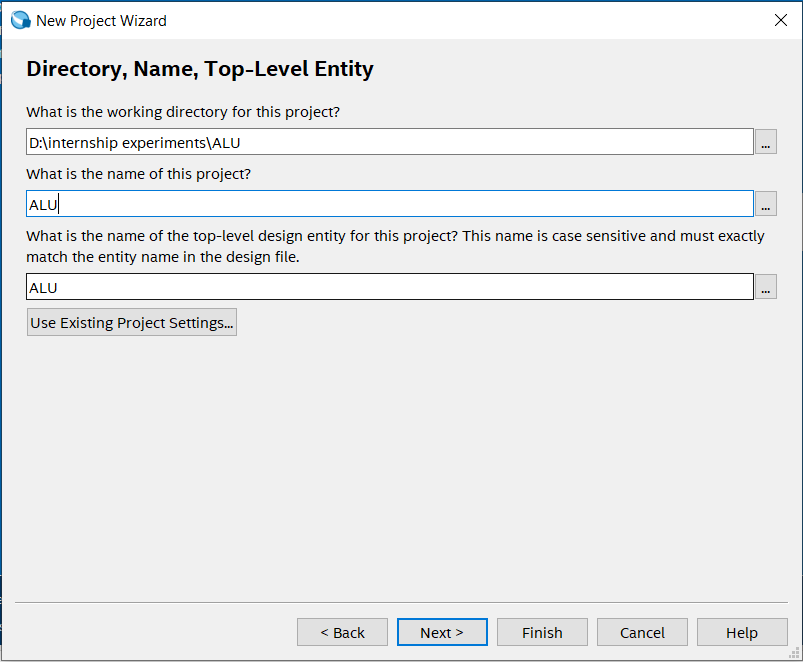
\includegraphics[width=14cm,keepaspectratio]{PRO IMG1.png}
    \caption{Creating New Project}
    \end{figure}
    
    \newpage
    \item You will see this screen after completing all steps. For detailed steps refer the \textbf{'Quick Start Guide to Quartus and ModelSim Software'} document.
    \newline
    \textbf{Note:} We will be using DE0 Nano Board (Cyclone IV Family EP4CE22F17C6) for entire project.
    \begin{figure}[H]
    \centering
    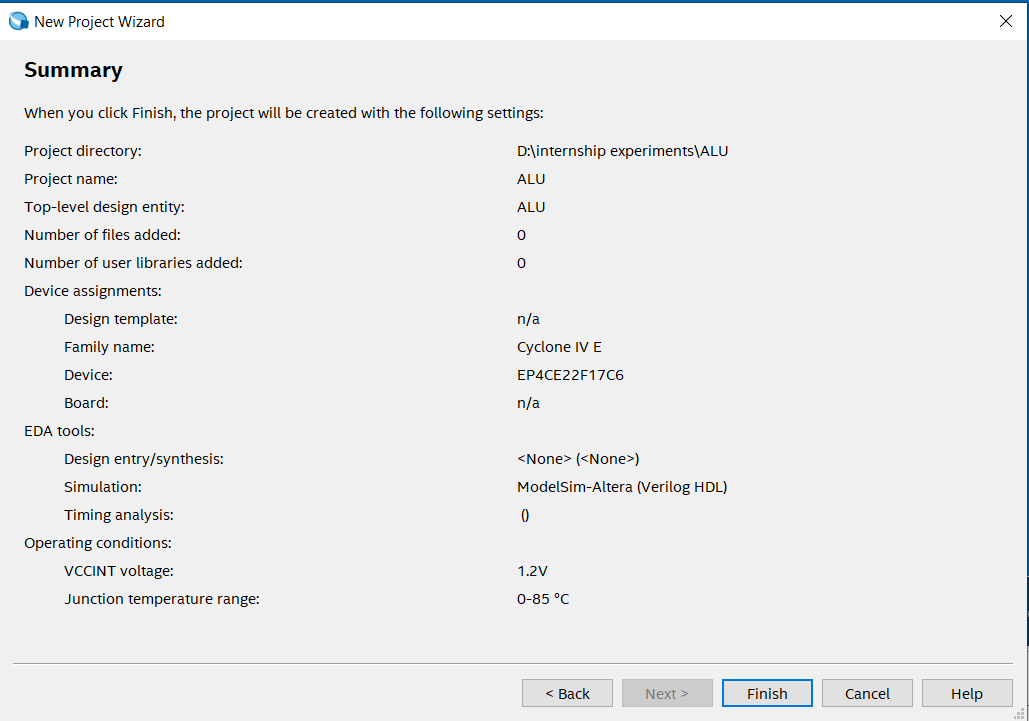
\includegraphics[width=14cm,keepaspectratio]{projimg2.png}
    \caption{Summary}
    \end{figure}
    
    \item We will be using \textbf{Verilog} throughout this project. Create a \textbf{New Verilog HDL file}.
    \begin{figure}[H]
        \centering
    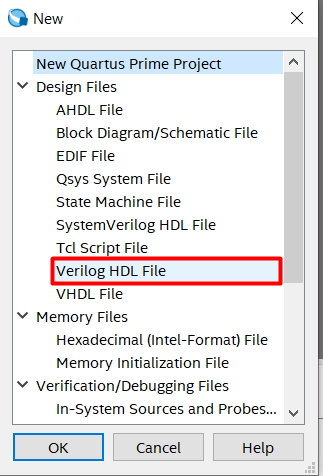
\includegraphics[scale =0.8]{PROJIMG3.png}
    \caption{New Verilog File}
    \end{figure}
    \newpage
    \item Type the code for 8-bit ALU(code on page 2) in this file.
    \begin{figure}[H]
        \centering
    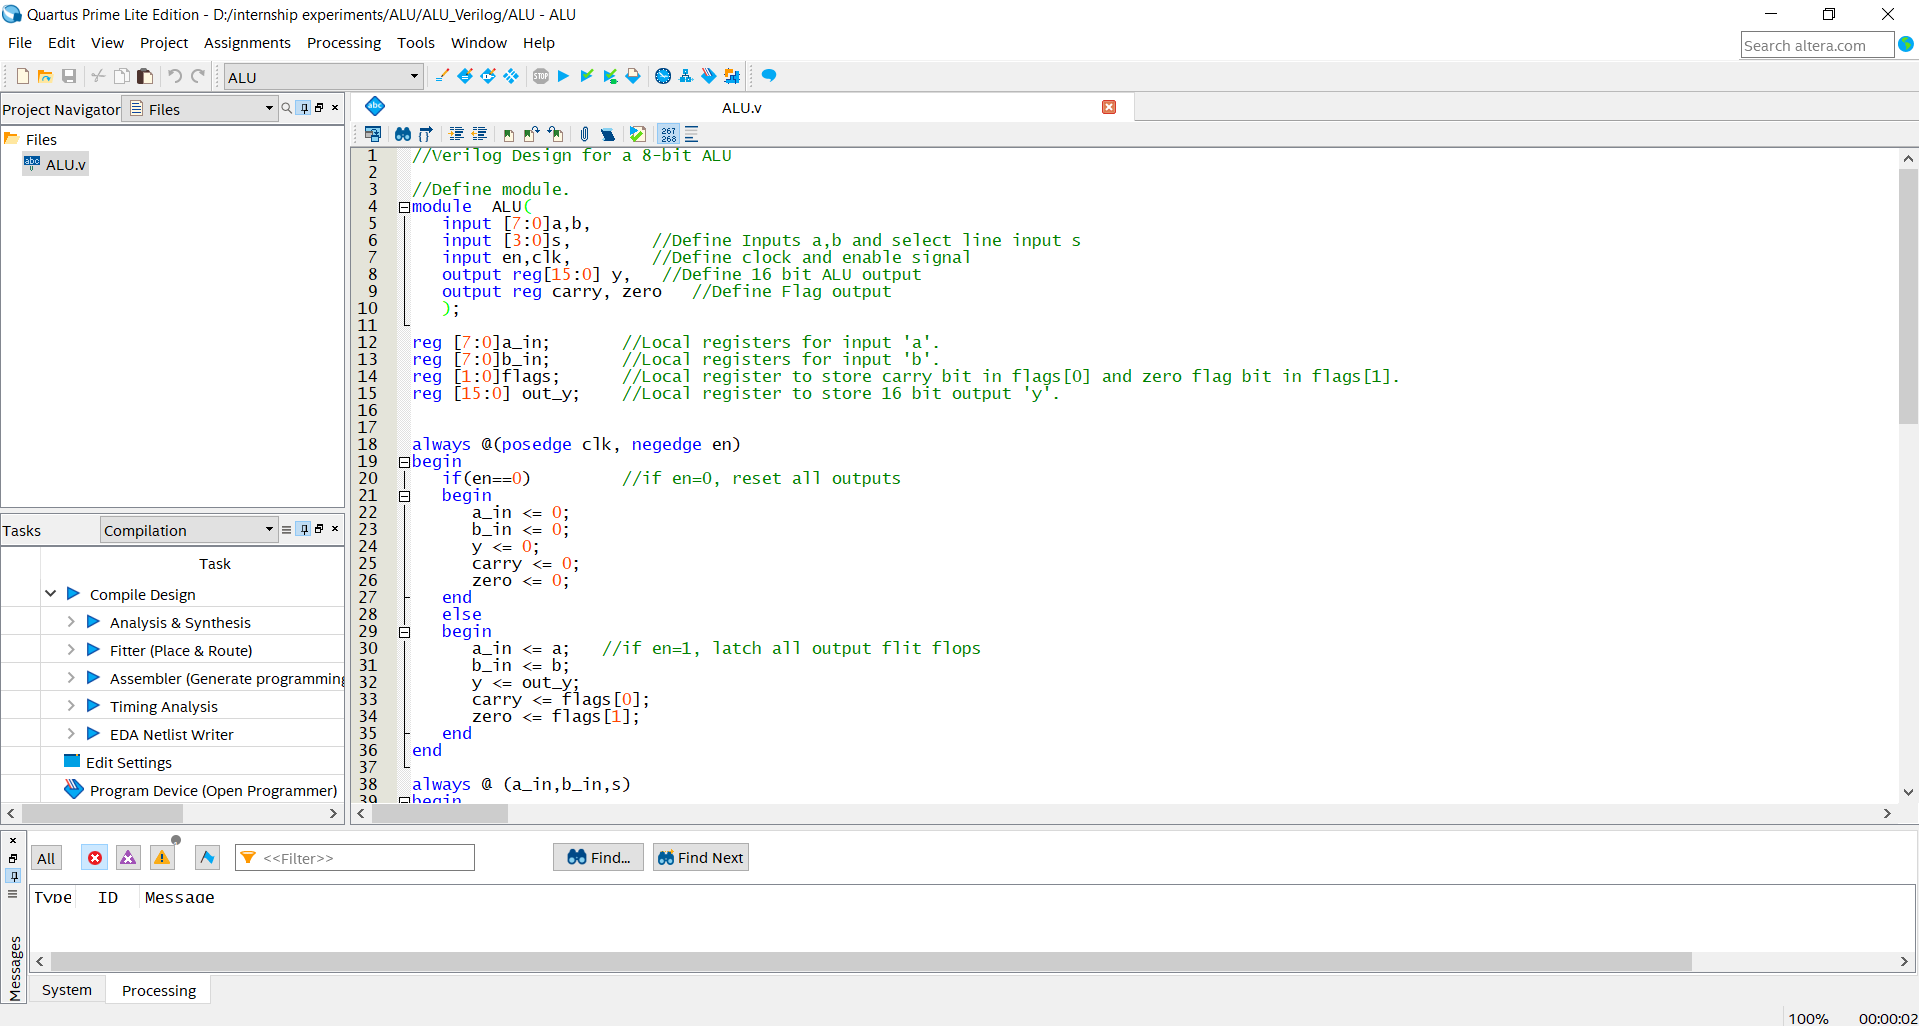
\includegraphics[width=14cm,keepaspectratio]{proentry.png}
    \caption{Verilog Code:ALU}
    \end{figure}
    
    \item Go to \textbf{File}$\rightarrow$\textbf{Save as} and save the file.\newline\textbf{Note:} File name should be same as module name.
    \begin{figure}[H]
        \centering
    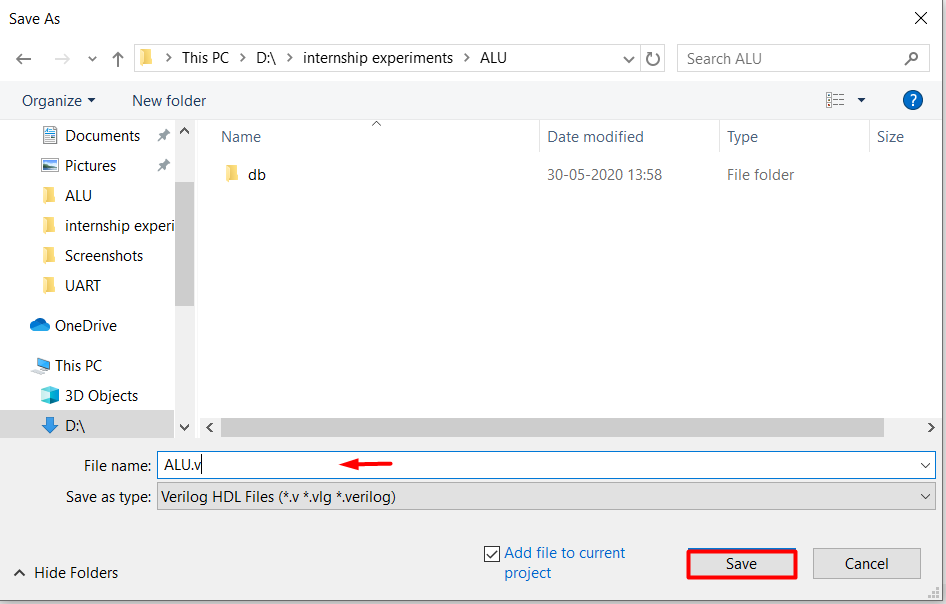
\includegraphics[width=14cm,keepaspectratio]{save4.png}
    \caption{Saving the file}
    \end{figure}
    \newpage
    \item Goto \textbf{Project}$\rightarrow$\textbf{Set as Top-Level Entity}. The \textbf{ALU} file is our main file and make sure you have selected this file while setting the top level entity.
    \begin{figure}[H]
        \centering
    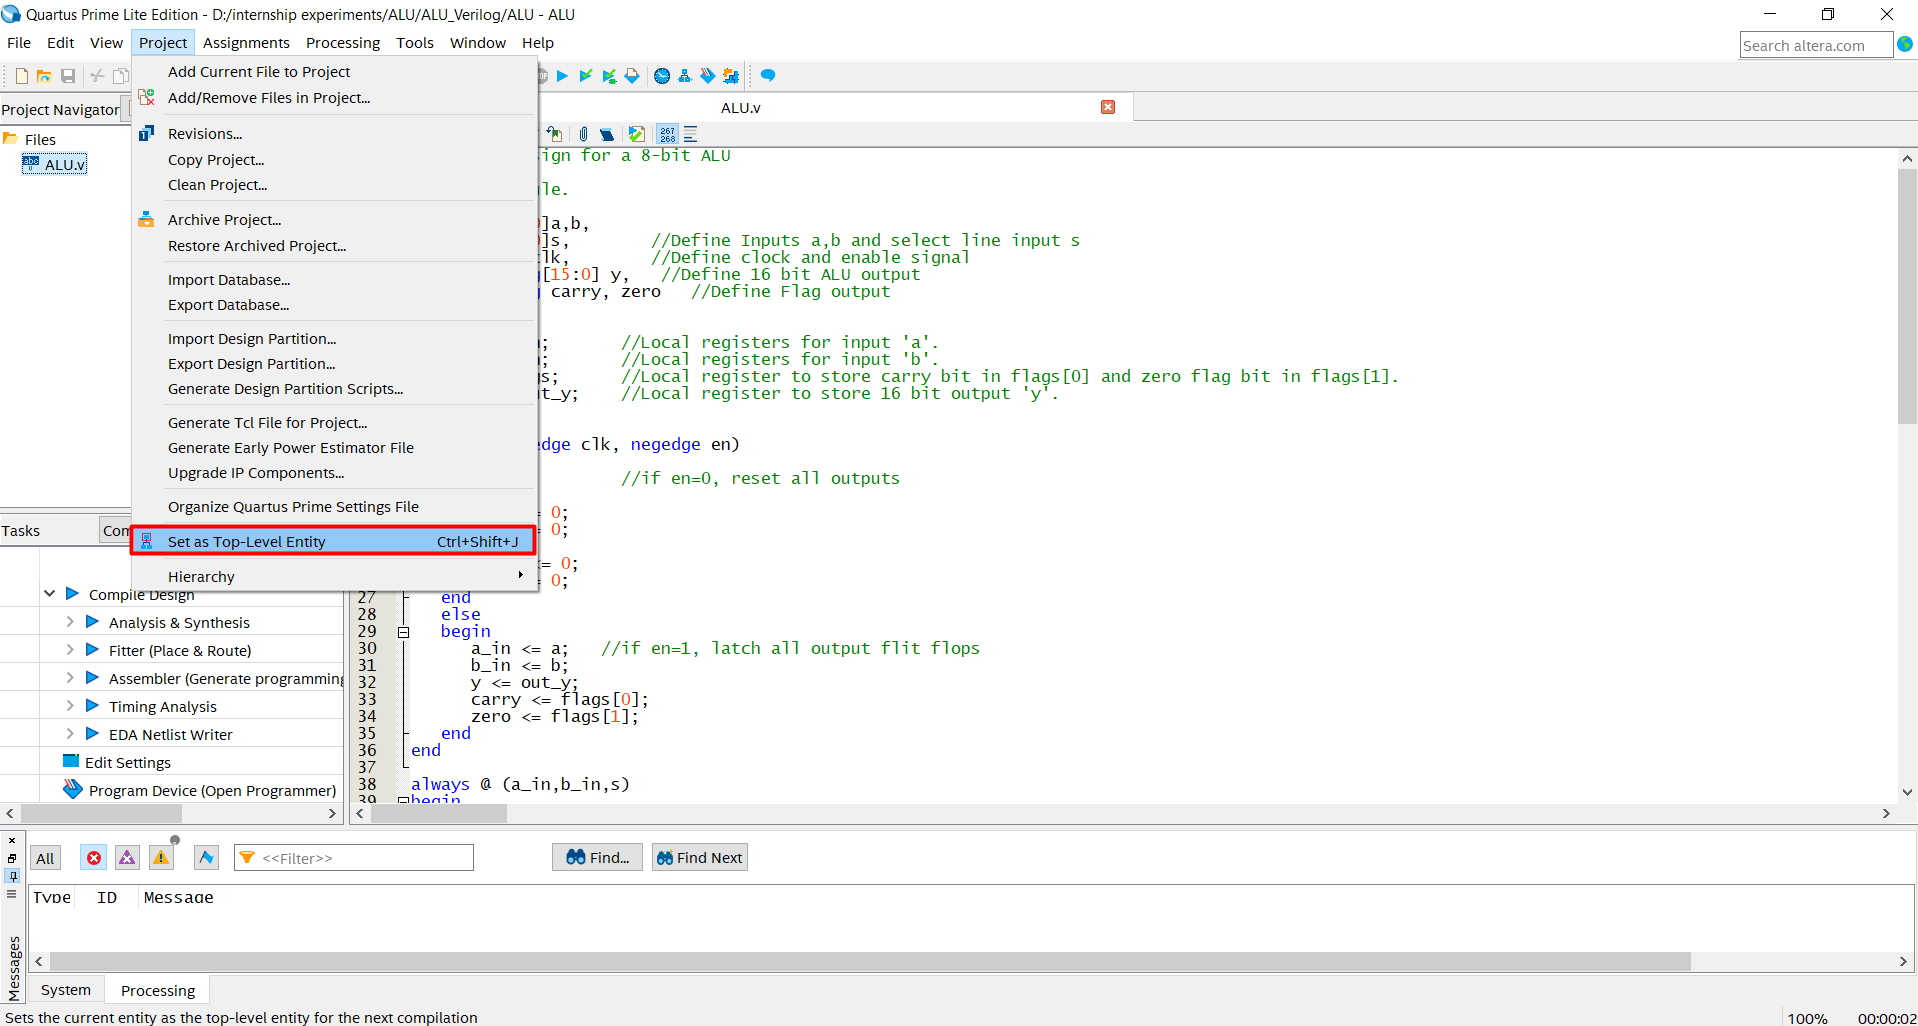
\includegraphics[width=14cm,keepaspectratio]{alusetnew2.png}
    \caption{Setting Top level entity}
    \end{figure}
    
    \item Goto \textbf{Processing}$\rightarrow$\textbf{Start Compilation}.
    \begin{figure}[H]
        \centering
    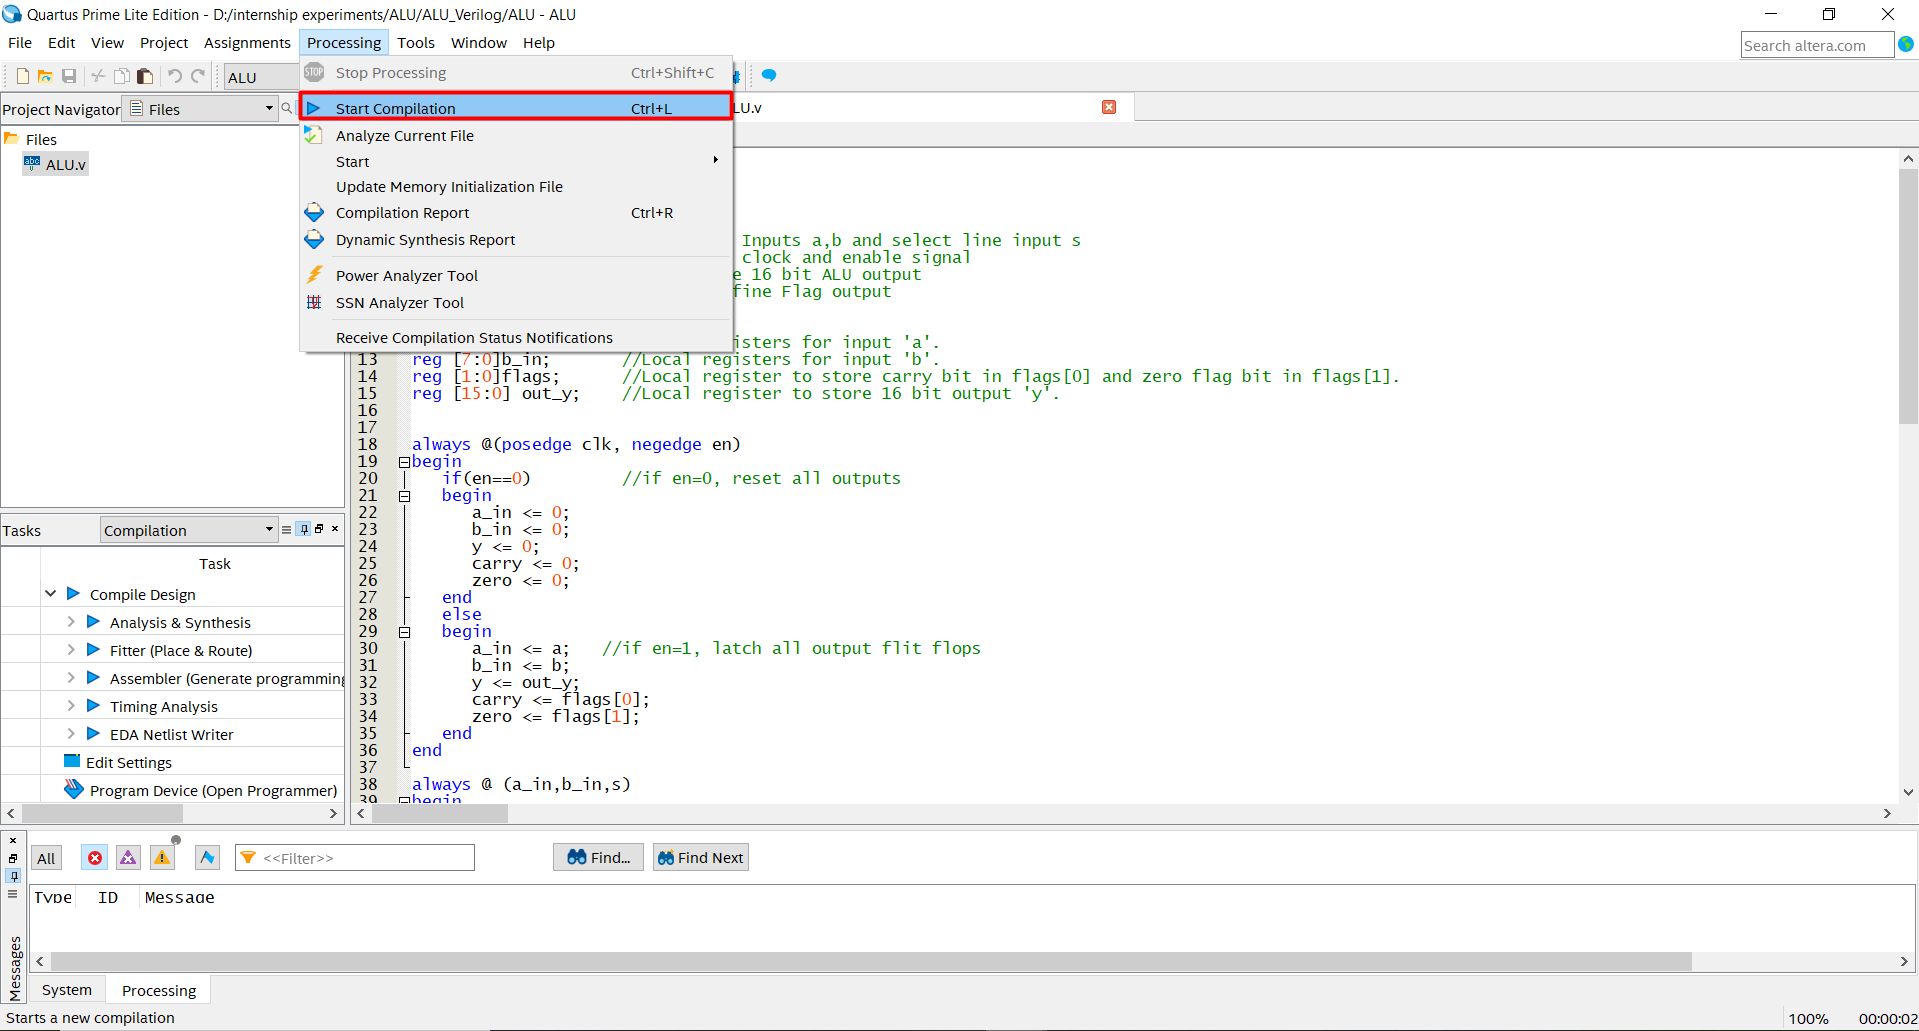
\includegraphics[width=14cm,keepaspectratio]{startcompialu.png}
    \caption{Compiling the Design}
    \end{figure}
    \newpage
    \item You can verify whether all the files are compiled successfully by checking the highlighted tabs i.e. \textbf{Messages} and \textbf{Tasks} tab.
    \begin{figure}[H]
        \centering
    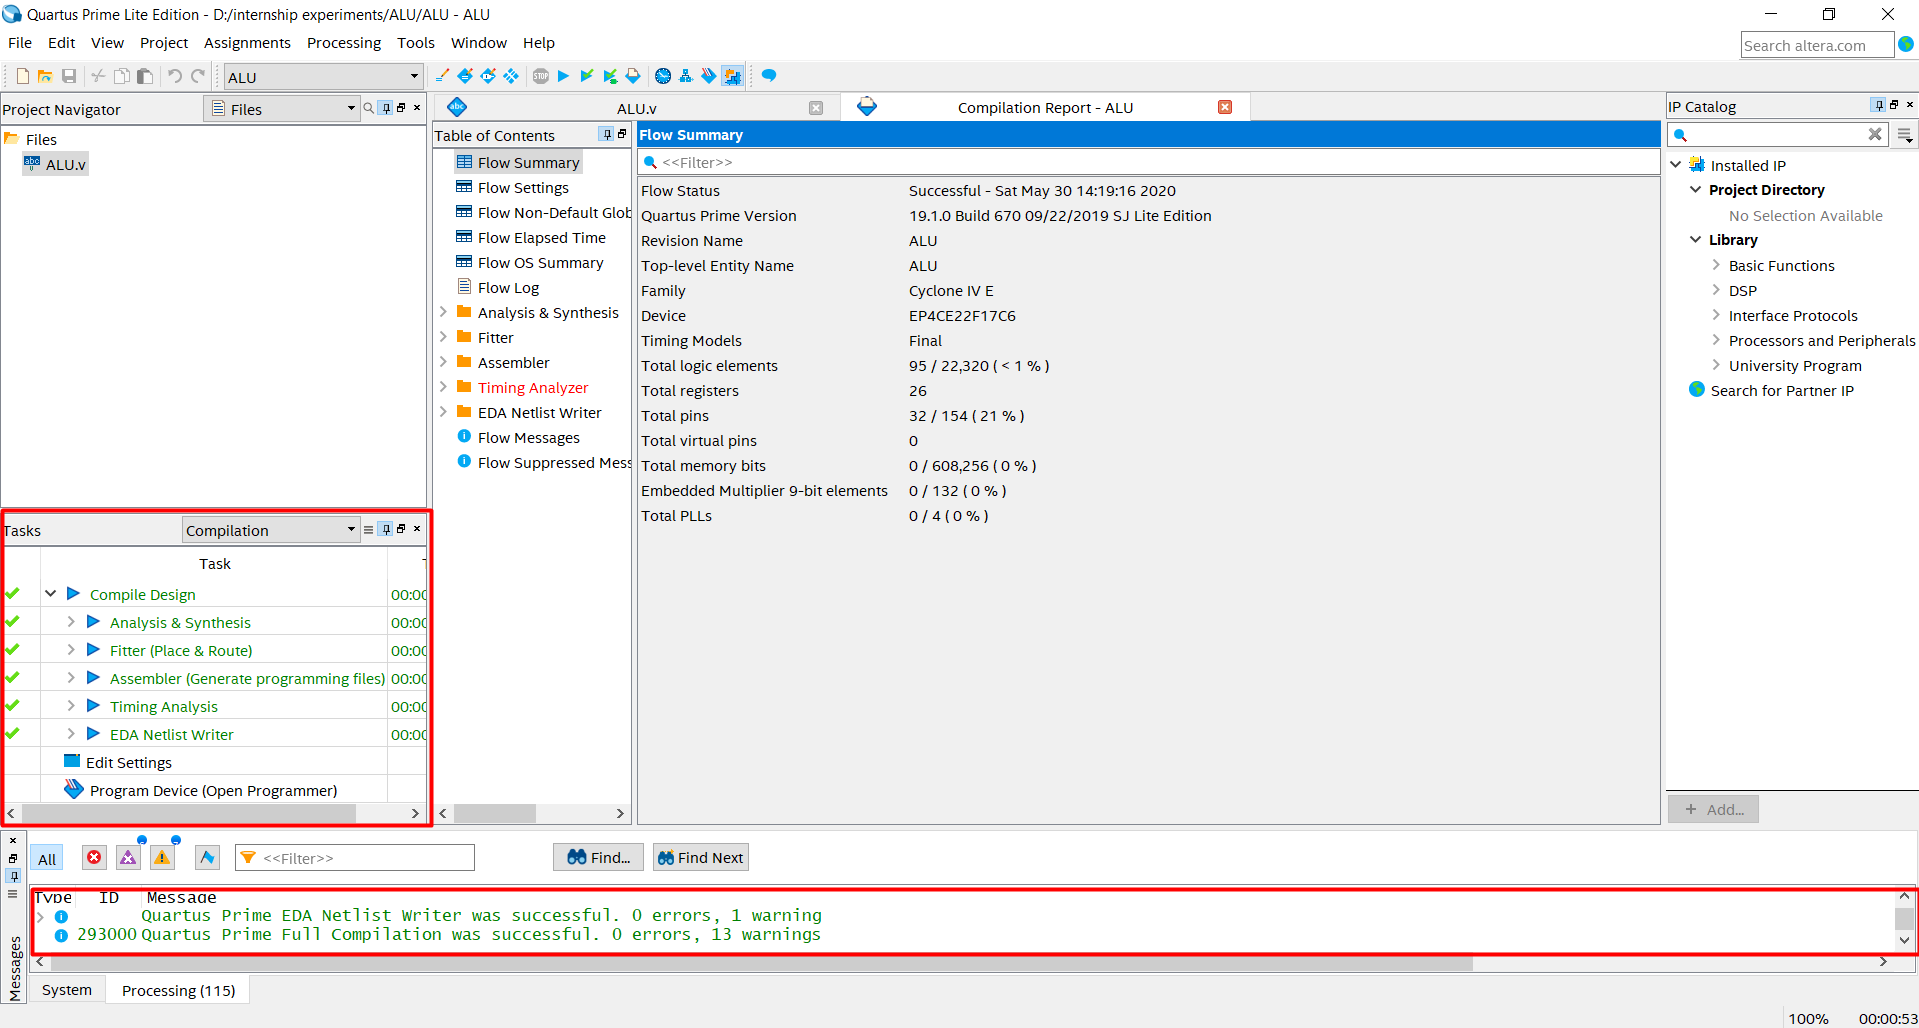
\includegraphics[width=14cm,keepaspectratio]{compilation done.png}
    \caption{Verification(Flow Summary)}
    \end{figure}
    
\end{enumerate}
\newpage
\section{RTL Circuit of the implemented design}
    \subsubsection*{Steps to get RTL circuit.}
        \begin{enumerate}
            \item Goto \textbf{Tools}$\rightarrow$\textbf{Netlist Viewers}$\rightarrow$\textbf{RTL Viewer}.
                \begin{figure}[H]
                     \centering
                  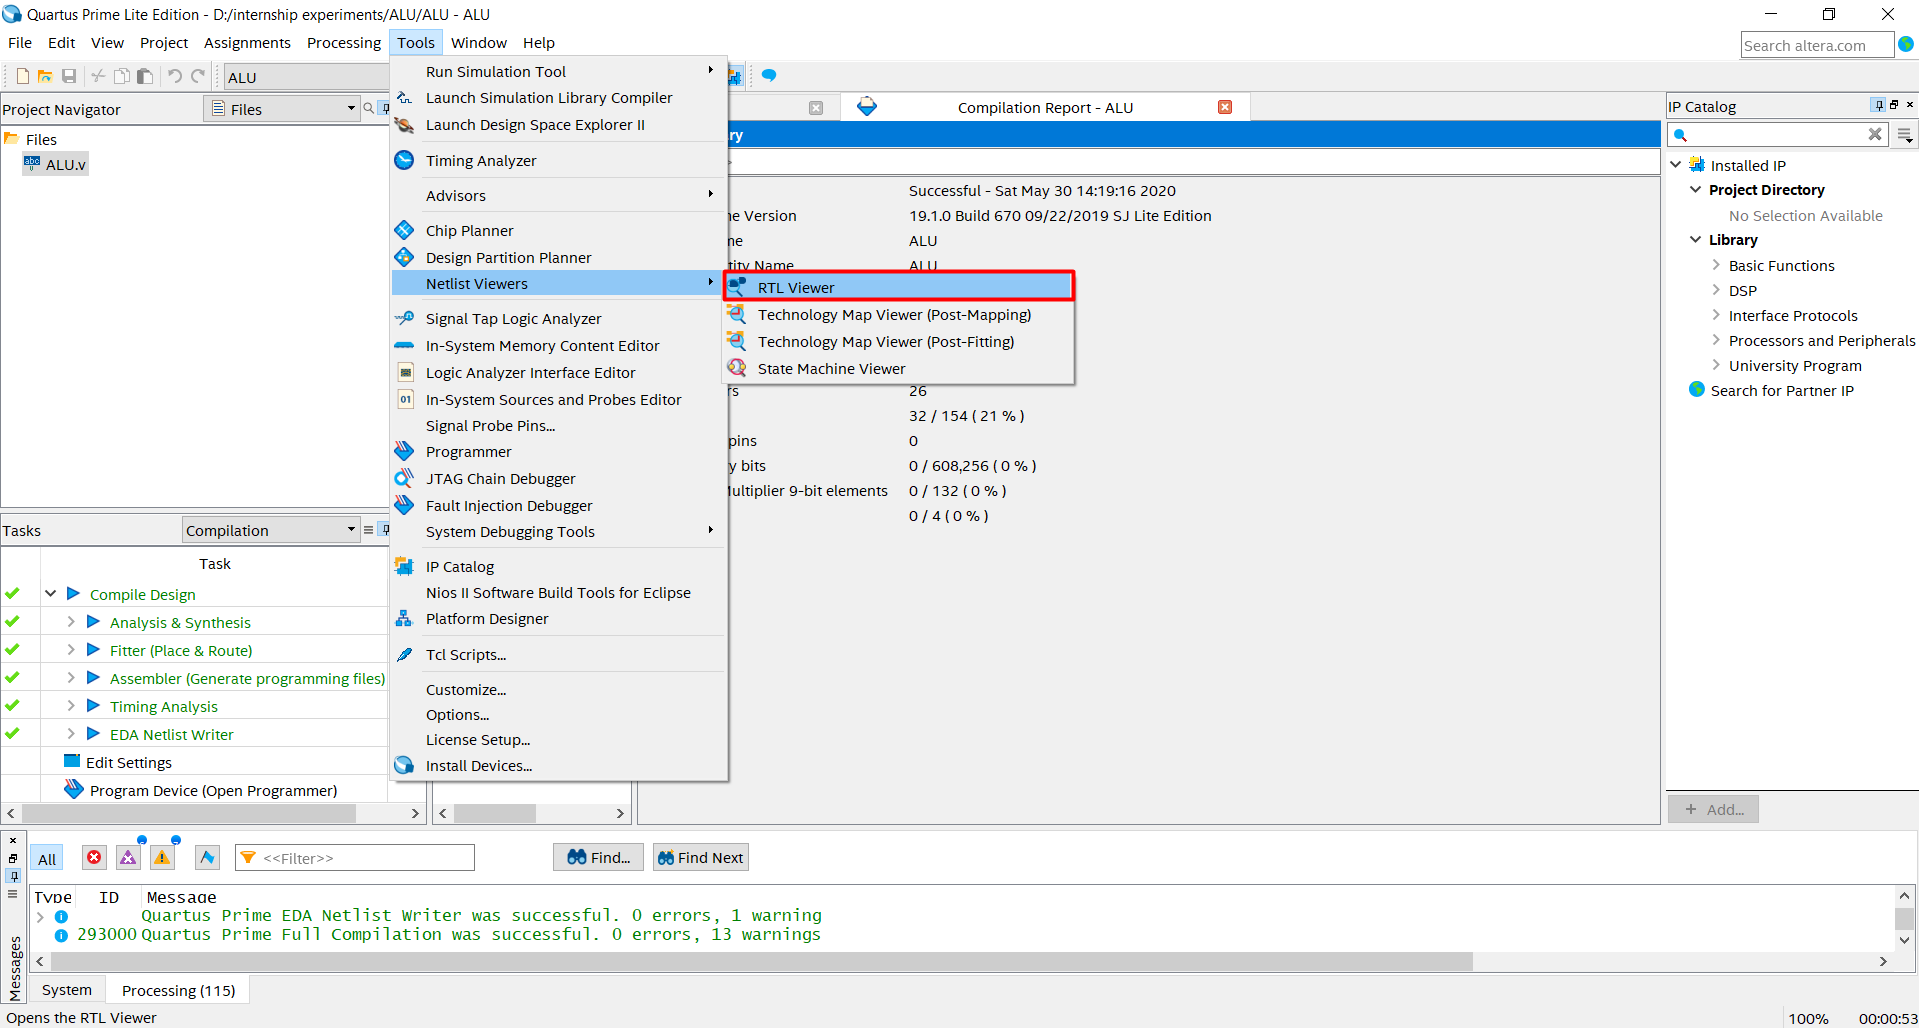
\includegraphics[scale=0.4]{rtl1.png}
                \caption{RTL Viewer}
                \end{figure}
            \item The below figure shows the equivalent RTL circuit of 8-bit ALU.      
\begin{figure}[H]
    \centering
    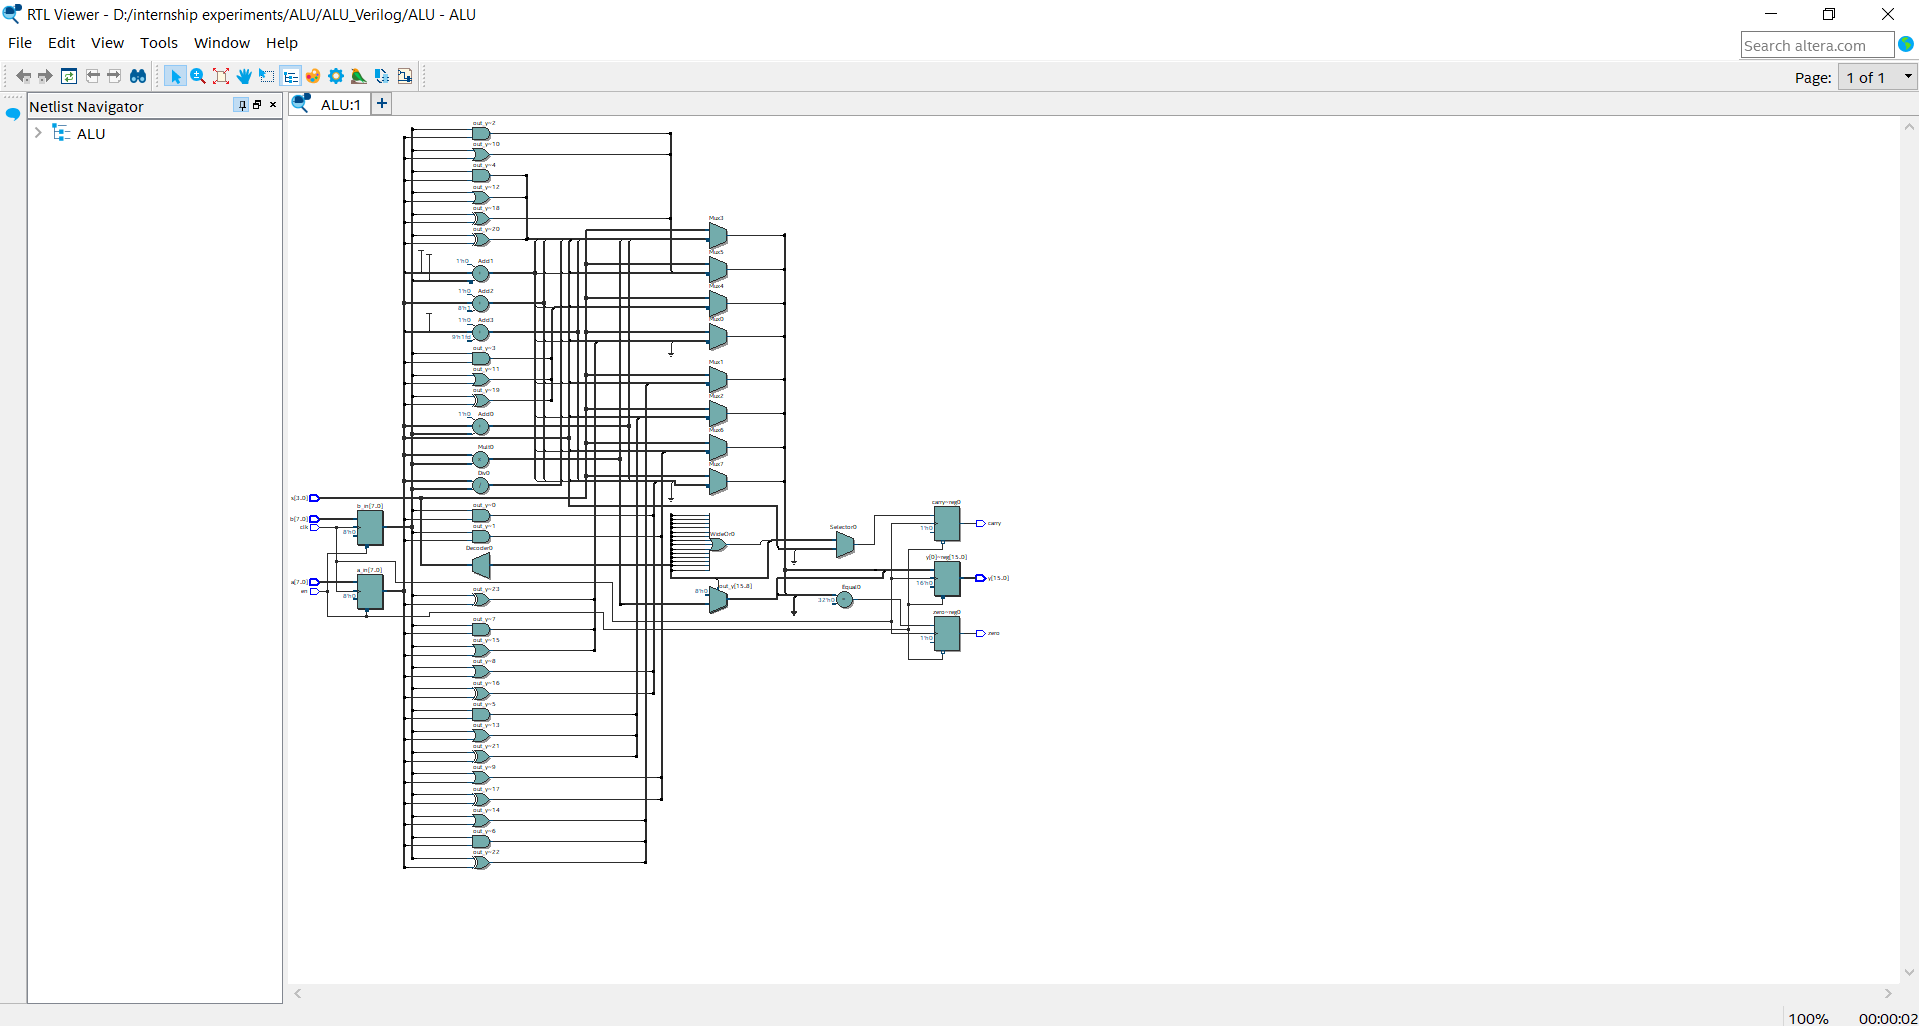
\includegraphics[scale=0.4]{rtlalu new.png}
    \caption{RTL Design for 8-bit ALU}
\end{figure}
\end{enumerate}

\newpage

 \section{Downloading the code to DE0 Nano FPGA Board}
 Before starting, Make sure the board is powered ON and connected to the computer through an USB Cable
 
 \begin{enumerate}
     \item Compile the Project by double clicking on \textbf{Compile} or the \textbf{Play} button. This creates an SRAM object file(.SOF file). This file is used to program the Device
     \begin{figure}[H]
         \centering
         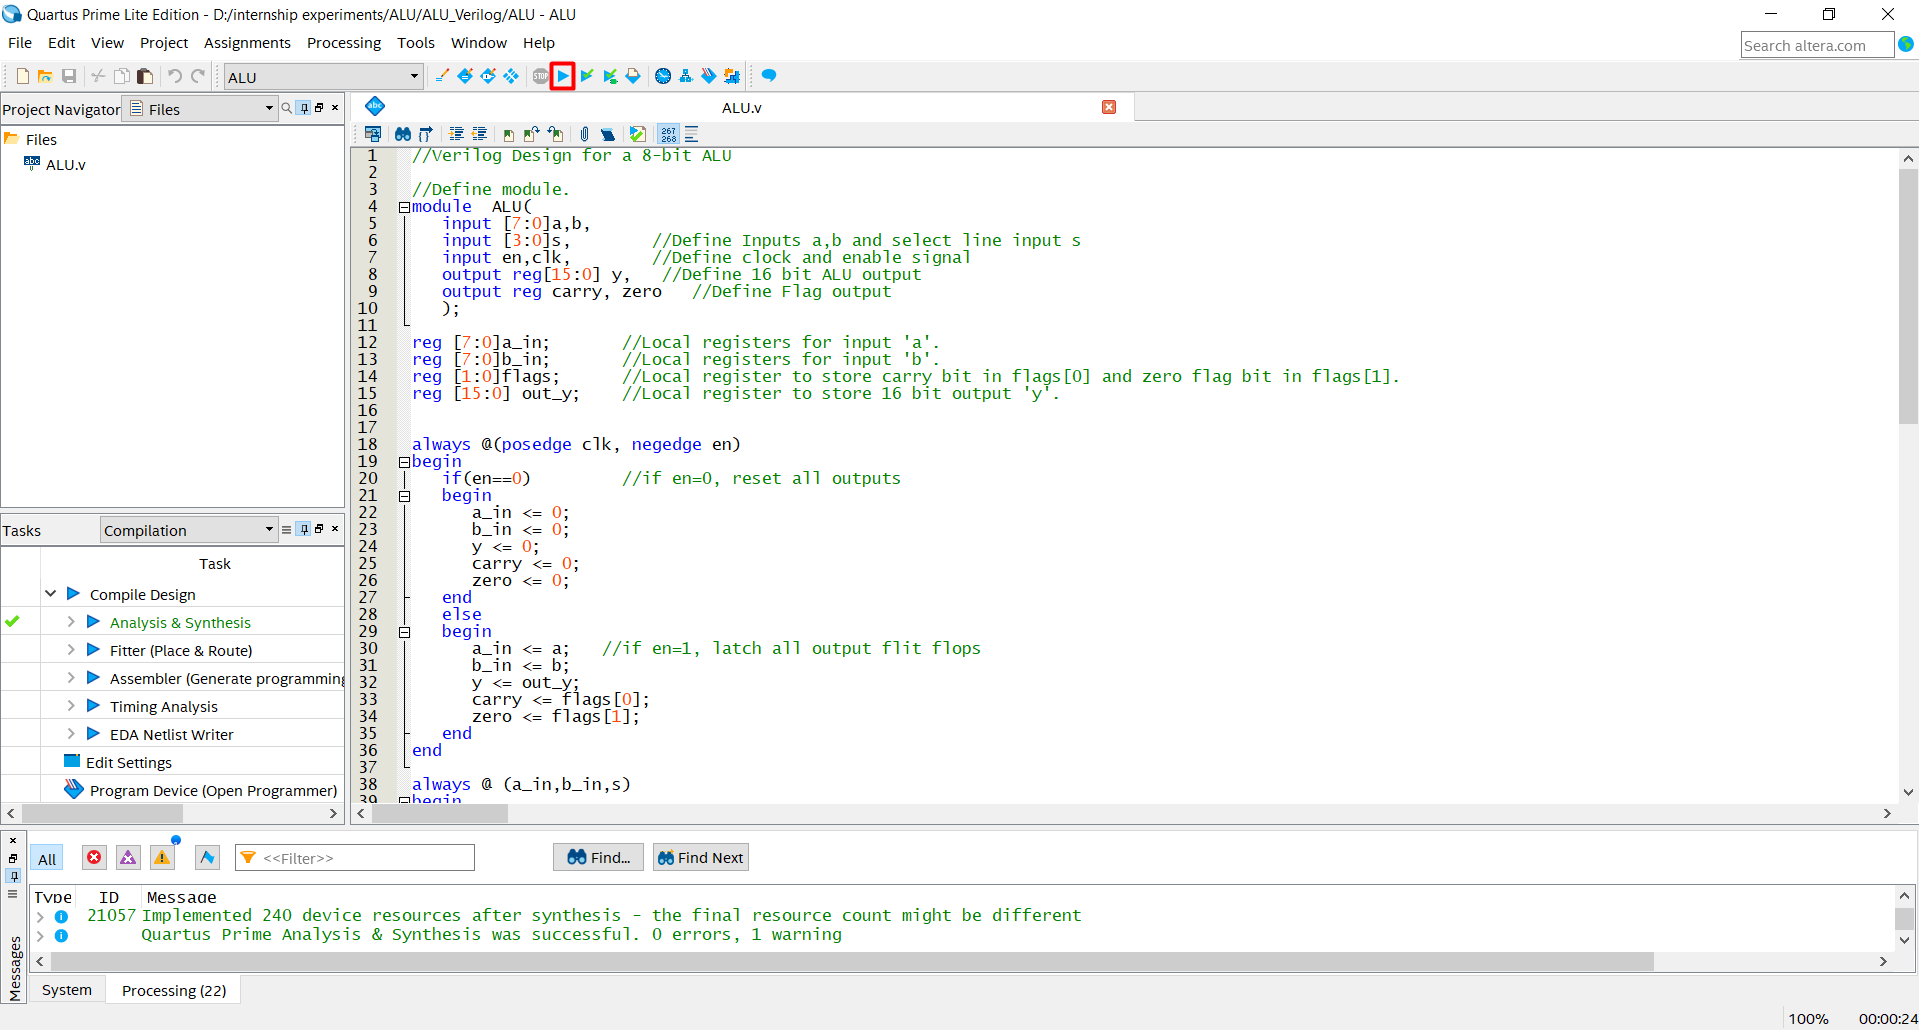
\includegraphics[width=14cm,keepaspectratio]{soffile.png}
     \caption{Creating .SOF file}
     \end{figure}
     
     \item Open the programmer by going to \textbf{Tools}$\rightarrow$\textbf{Programmer}
     \begin{figure}[H]
         \centering
         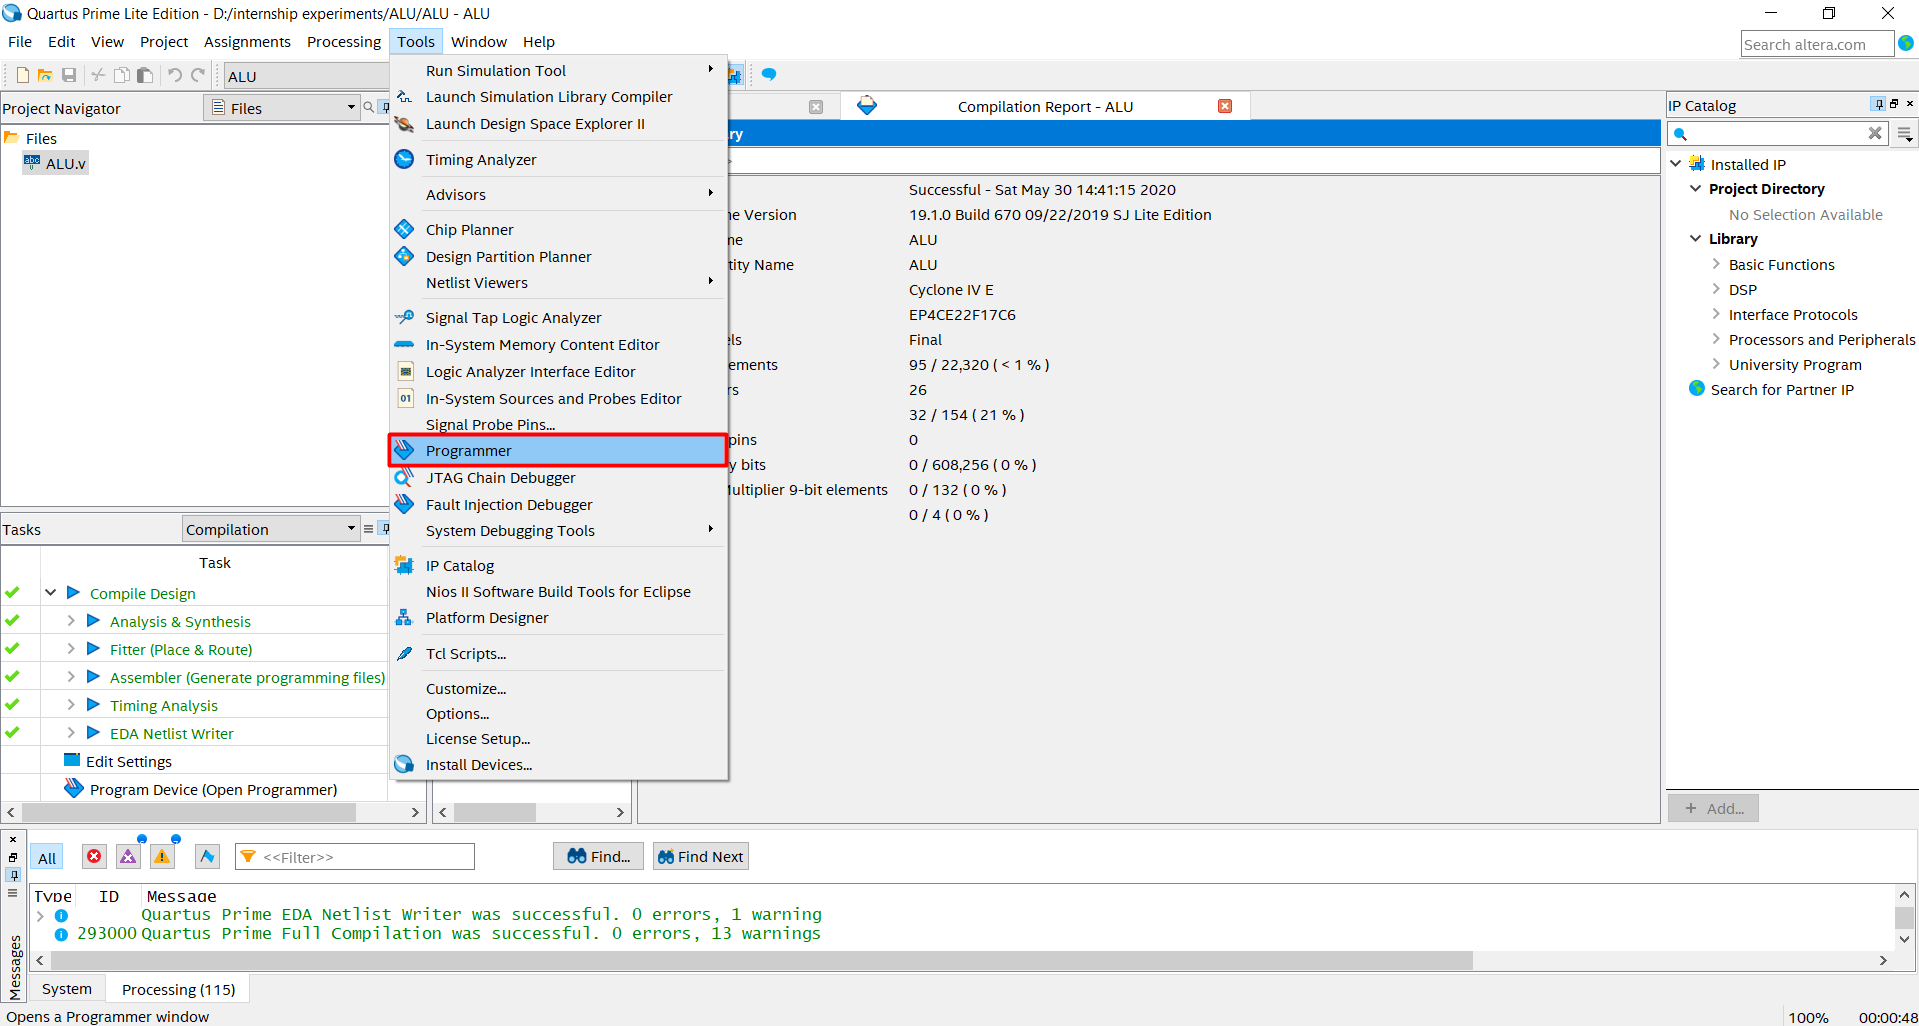
\includegraphics[width=14cm,keepaspectratio]{download2.png}
     \caption{Programmer}
     \end{figure}
     \newpage
     
     \item Click on \textbf{Hardware Setup}. The Device required must be listed under "Currently available hardware". If not, check if the device drivers are correctly installed. Choose the hardware from the dropdown menu
     \begin{figure}[H]
         \centering
         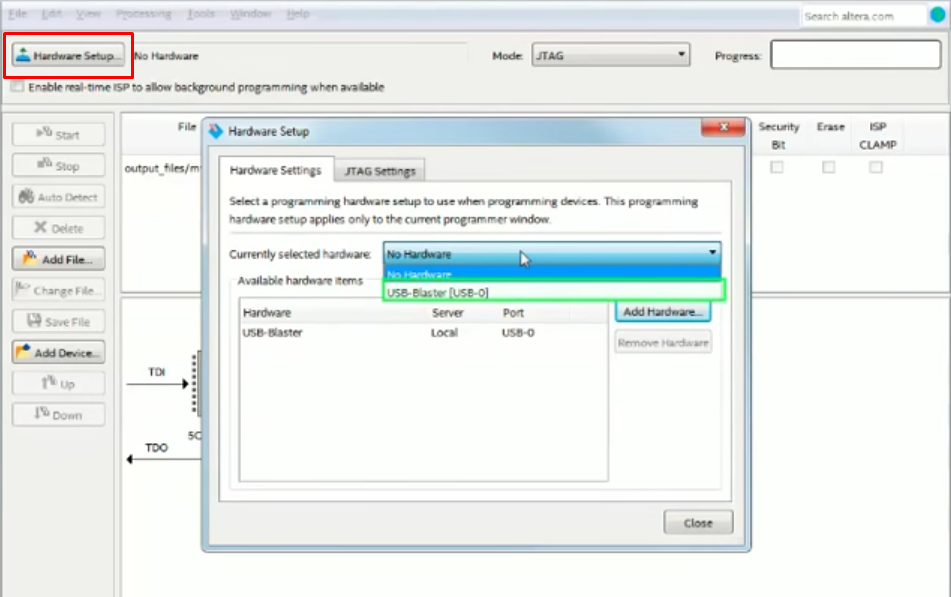
\includegraphics[scale=0.6]{3.png}
     \caption{Hardware setup}
     \end{figure}
     
     \item If the file is not listed, it can be manually added by clicking on \textbf{Add File}. The .SOF file can be found in the output directory inside the project directory 
     \begin{figure}[H]
         \centering
         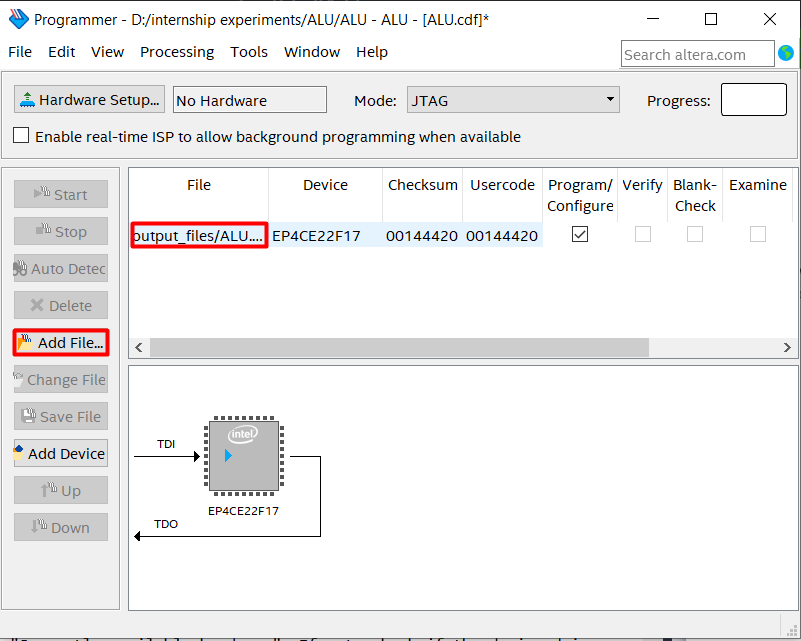
\includegraphics[scale=0.6]{download4.png}
     \caption{Add file}
     \end{figure}
     \newpage
     \item Make sure the Program/Configure checkbox is ticked
     \begin{figure}[H]
         \centering
         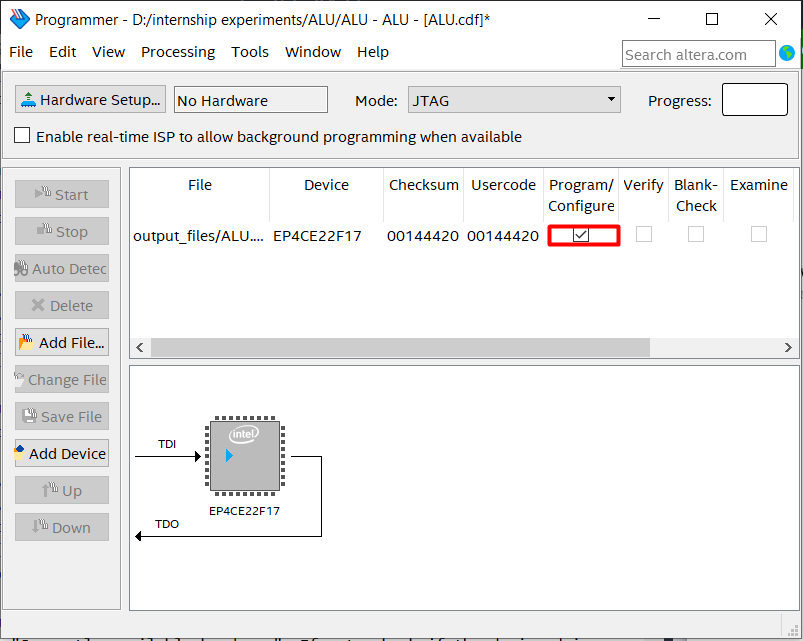
\includegraphics[width=14cm,keepaspectratio]{download5.png}
     \caption{Setting Program Configure}
     \end{figure}
     
     \item When ready, click on \textbf{Start} to start the programming process. \textbf{Start} button will be enabled when the 'DEO NANO' board is connected to USB port of your device. 
     \begin{figure}[H]
         \centering
         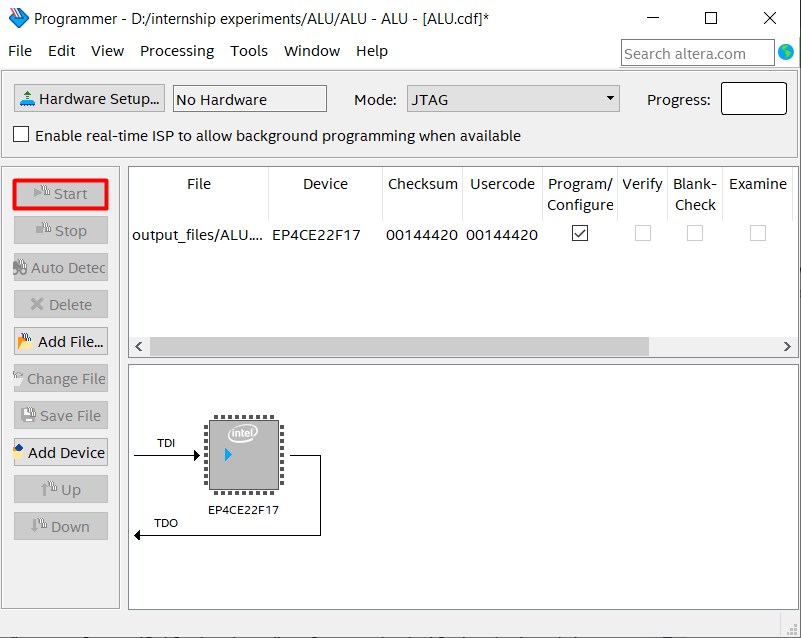
\includegraphics[height=7cm,keepaspectratio]{download6.png}
     \caption{Initiating Design Download into FPGA}
     \end{figure}
     
 \end{enumerate}
\newpage
\section{Implementing on Modelsim }
For more detailed procedure on using ModelSim, refer \textbf{Quick Start Guide to Quartus and ModelSim Software} Document. You can find both Verilog HDL and VHDL TestBench code below, make sure to follow only one language in this entire tutorial.

 \begin{enumerate}
     \item Create a New Verilog file in Quartus Prime.Type in the TestBench code provided in this document and save the file with the same name as the module name
    \begin{figure}[H]
        \centering
    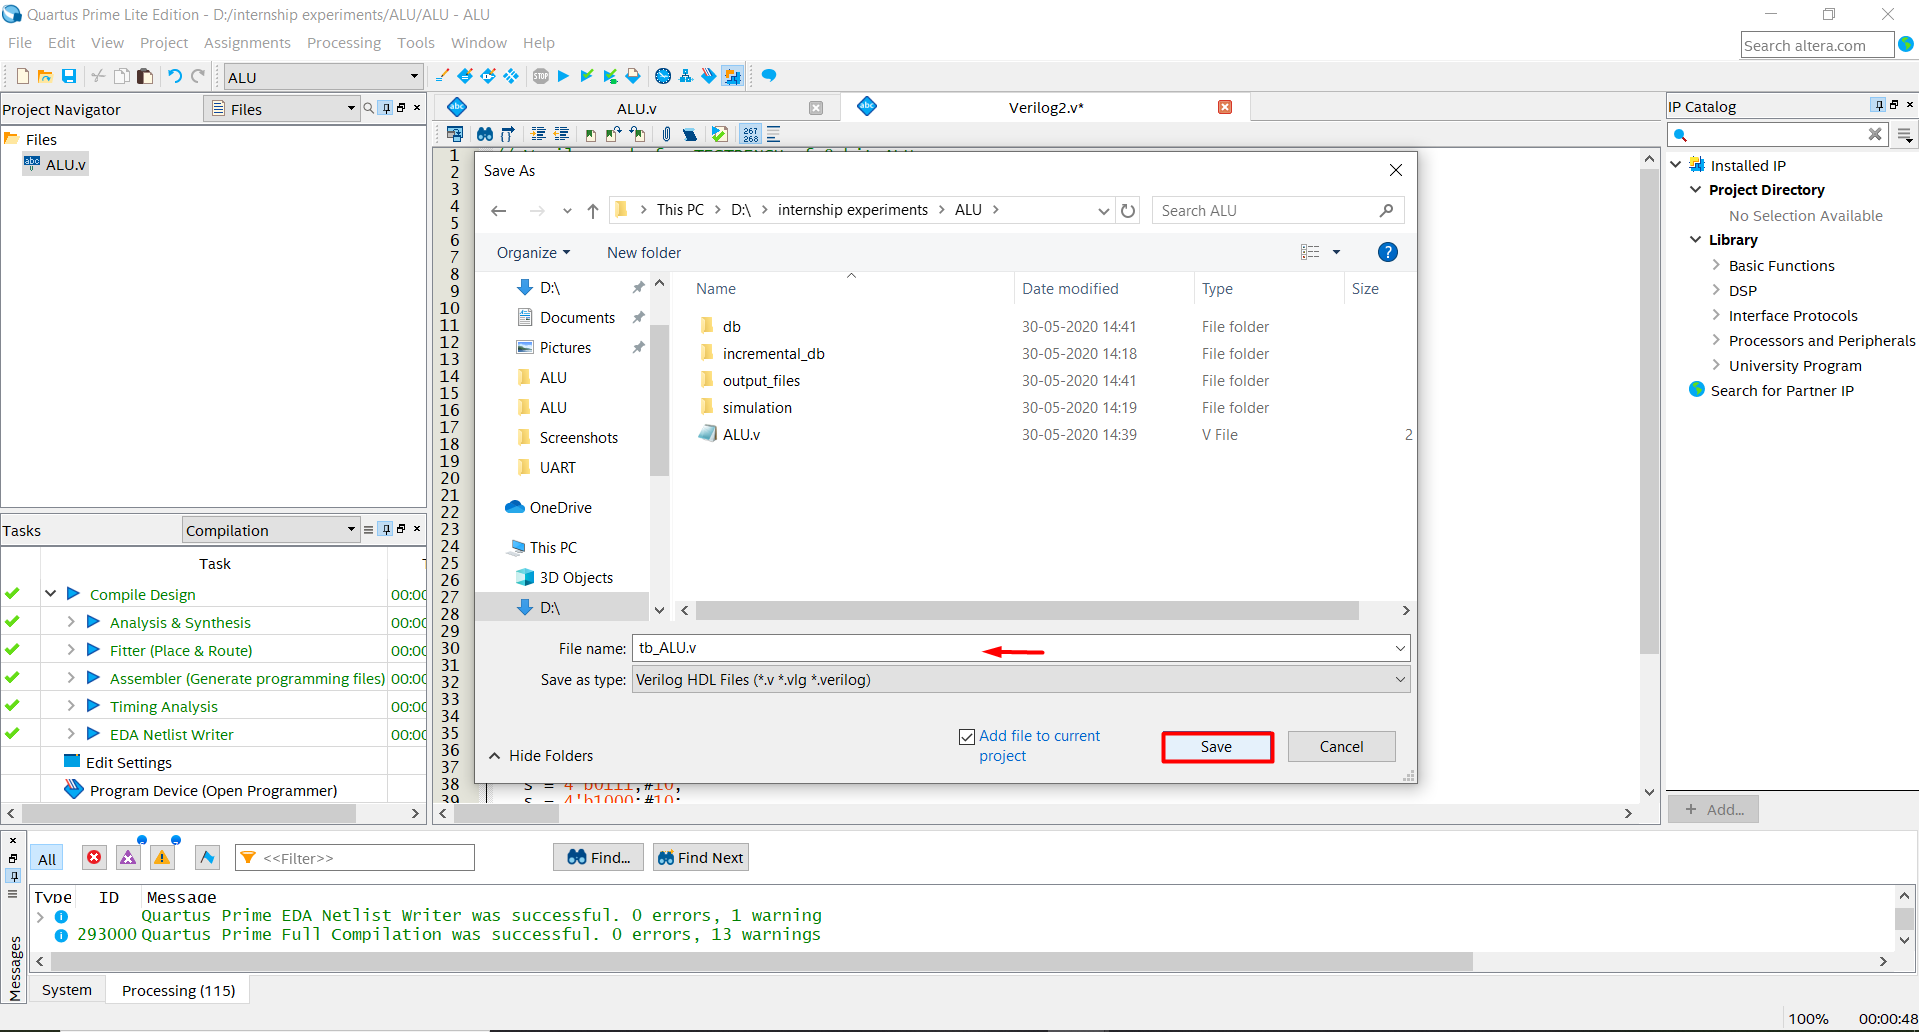
\includegraphics[width=14cm,keepaspectratio]{test1.png}
    \caption{Save TestBench file}
    \end{figure}
   
    \item Go to \textbf{Assignments}$\rightarrow$\textbf{Settings}.
    \begin{figure}[H]
        \centering
    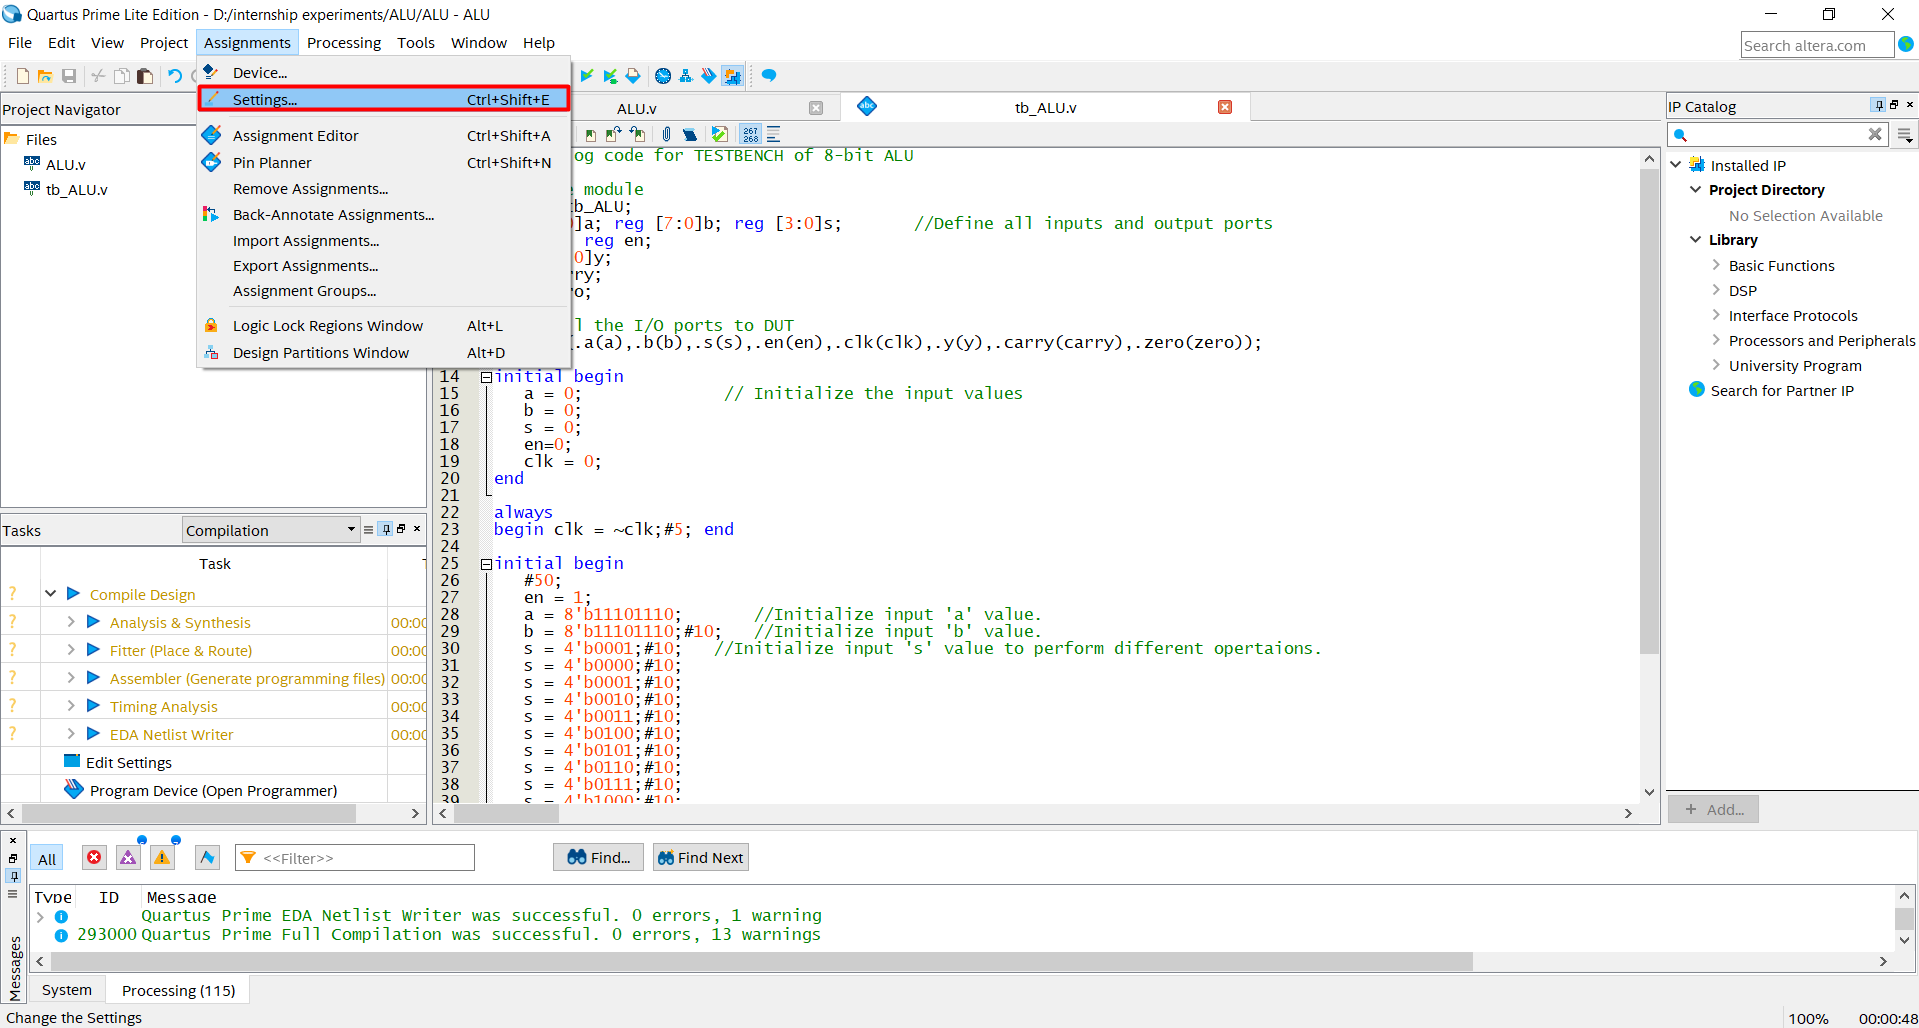
\includegraphics[width=14cm,keepaspectratio]{test2.png}
    \caption{Settings}
    \end{figure}
    \newpage
    \item Navigate to \textbf{Simulation} under \textbf{EDA Tool Settings}.Set the language as VHDL. Select \textbf{Compile TestBench} and then click on \textbf{Test Benches}.
    \begin{figure}[H]
        \centering
    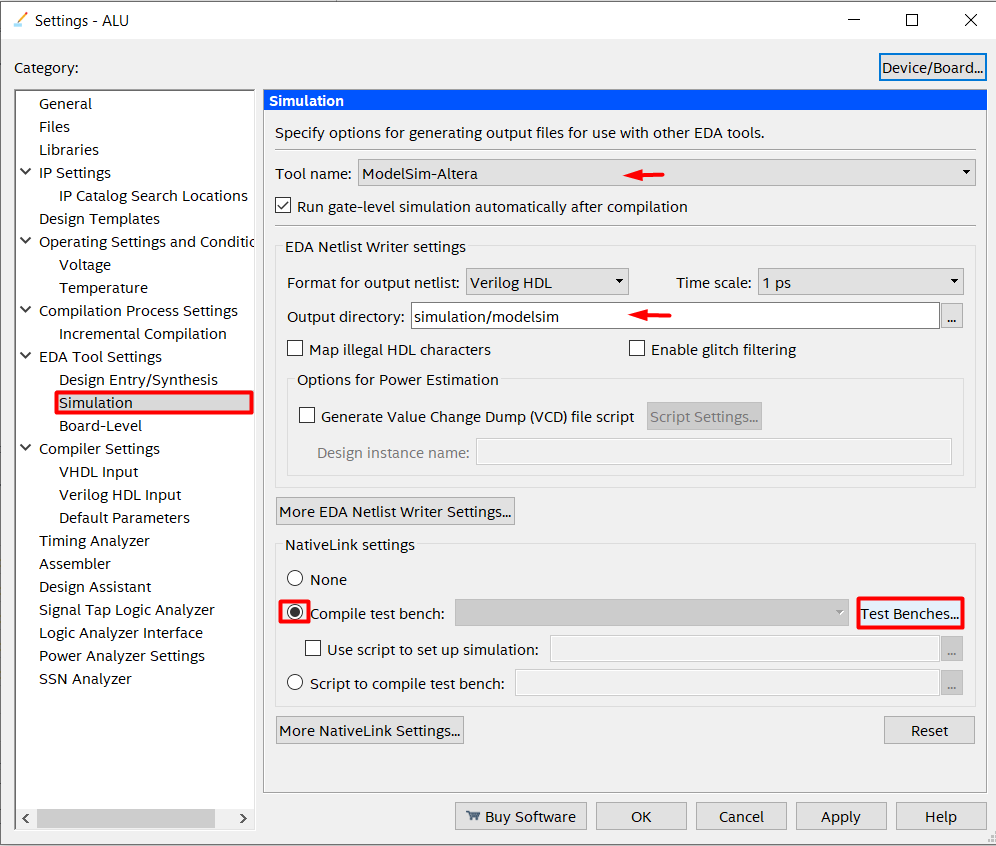
\includegraphics[width=14cm,keepaspectratio]{test3.png}
    \caption{Adding the TestBench file}
    \end{figure}
  
    \item Click on \textbf{New}, this opens another dialogue box.
    \begin{figure}[H]
        \centering
    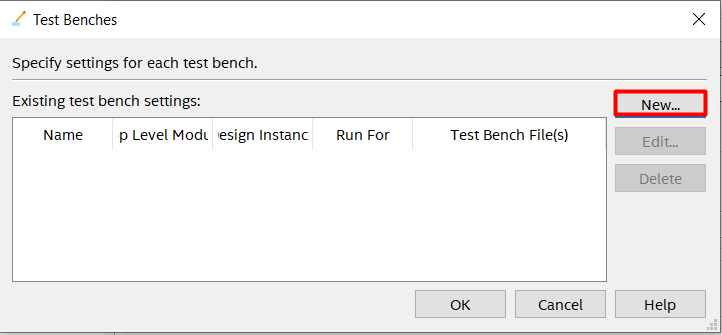
\includegraphics[width=14cm,keepaspectratio]{test4.png}
    \caption{Adding the TestBench file}
    \end{figure}
    \newpage
    \item Now type in the TestBench name(In this design , its \textbf{tb\_ripple\_carry\_adder}). Now click on the highlighted Browse button.Find the TestBench file(it can be found in the project directory) and click on \textbf{Open}. Now click on \textbf{Add},then \textbf{OK}.
            \begin{figure}[H]
        \centering
    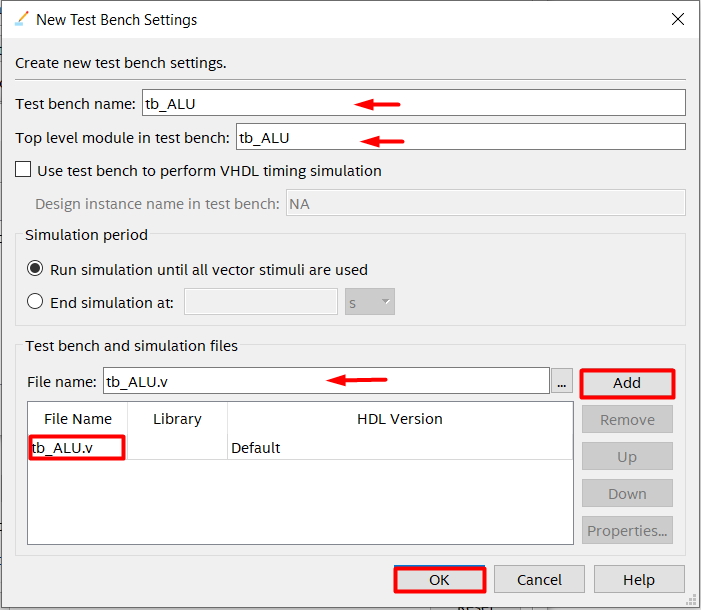
\includegraphics[scale=0.73]{test5.png}
    \caption{Adding the TestBench file}
    \end{figure}
    
 \end{enumerate}

 \noindent \textbf{Functional Simulation using NativeLink Feature}
    \begin{enumerate}
        
        \item  Go to \textbf{Processing}$\rightarrow$\textbf{Start Compilation}
            \begin{figure}[H]
                \centering
                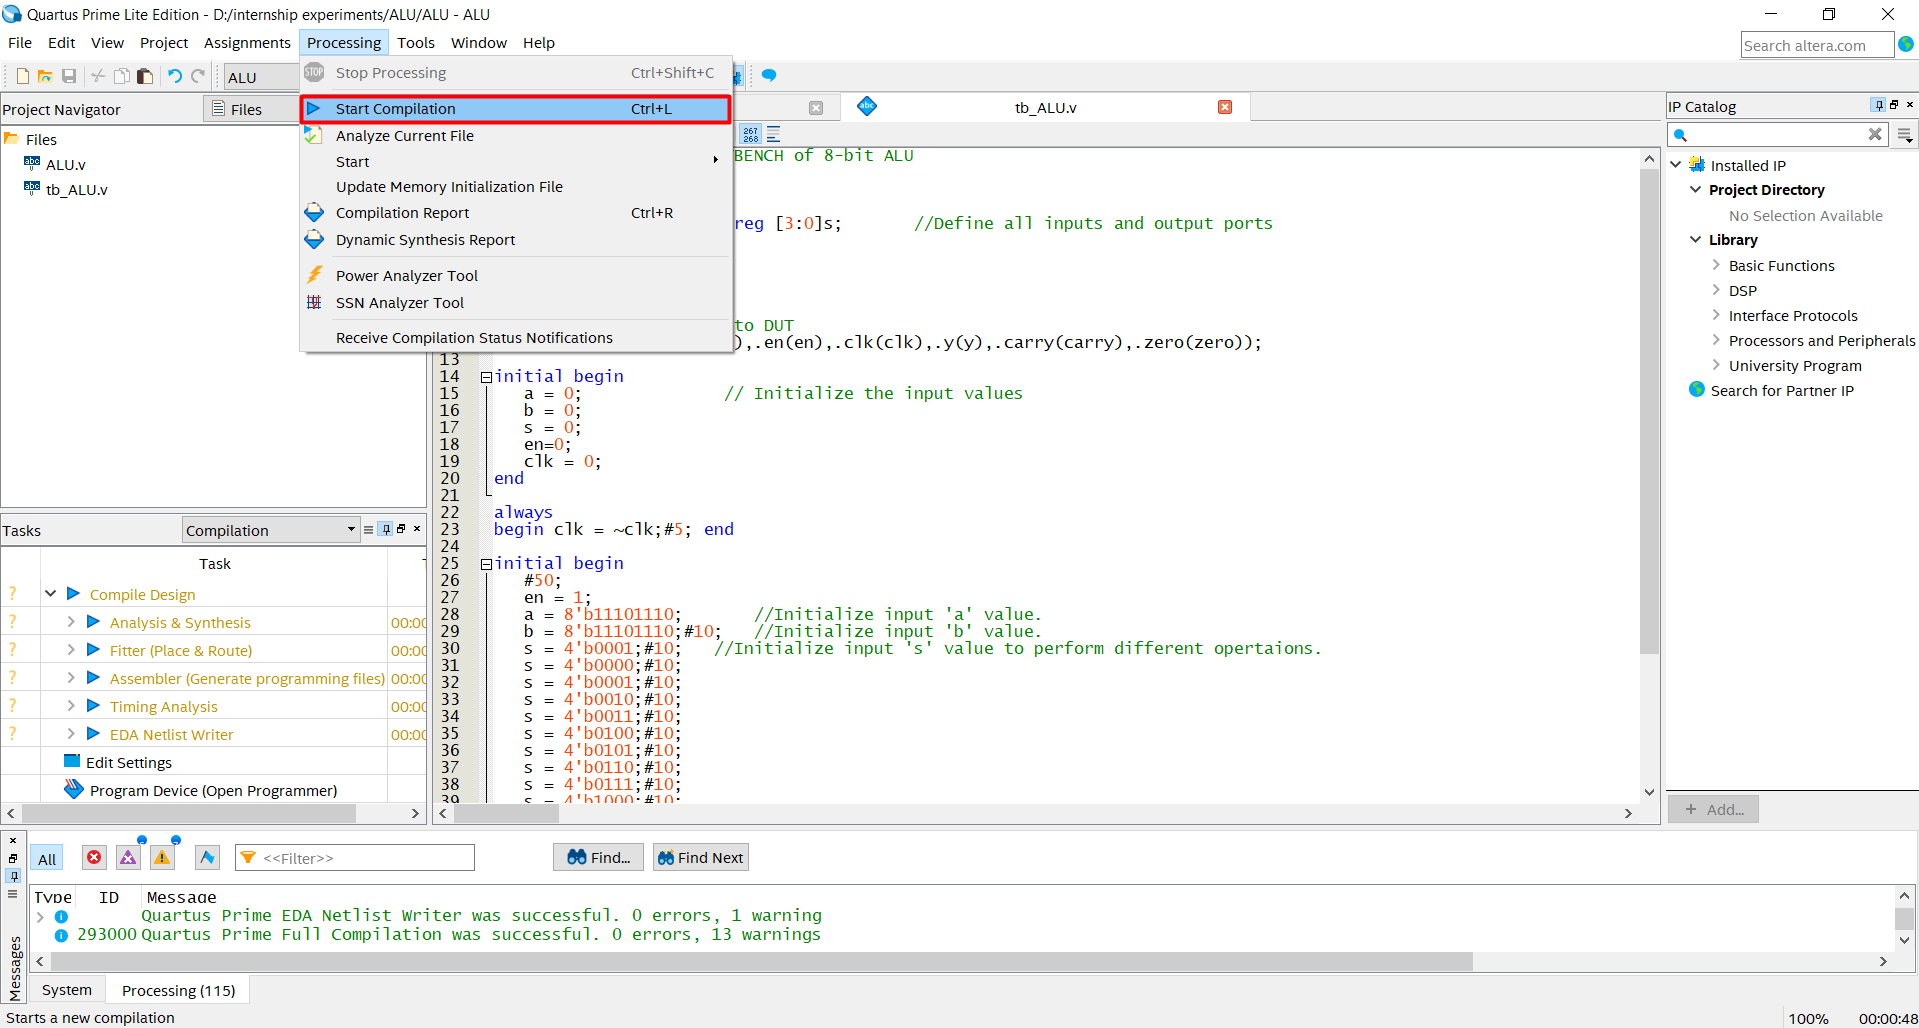
\includegraphics[width=14cm,keepaspectratio]{posttest1.png}
            \caption{Compiling the project}
            \end{figure}
    
        \newpage
        \item Go to \textbf{Tools}$\rightarrow$\textbf{Run Simulation Tool}$\rightarrow$\textbf{RTL Simulation} to automatically run the EDA simulator(ModelSim-Altera) and to compile all necessary design files.
        \newline\textbf{Note:} If you cannot see the graph, Click on the waveform window and select the \textbf{Zoom all} option.
            \begin{figure}[H]
                \centering
                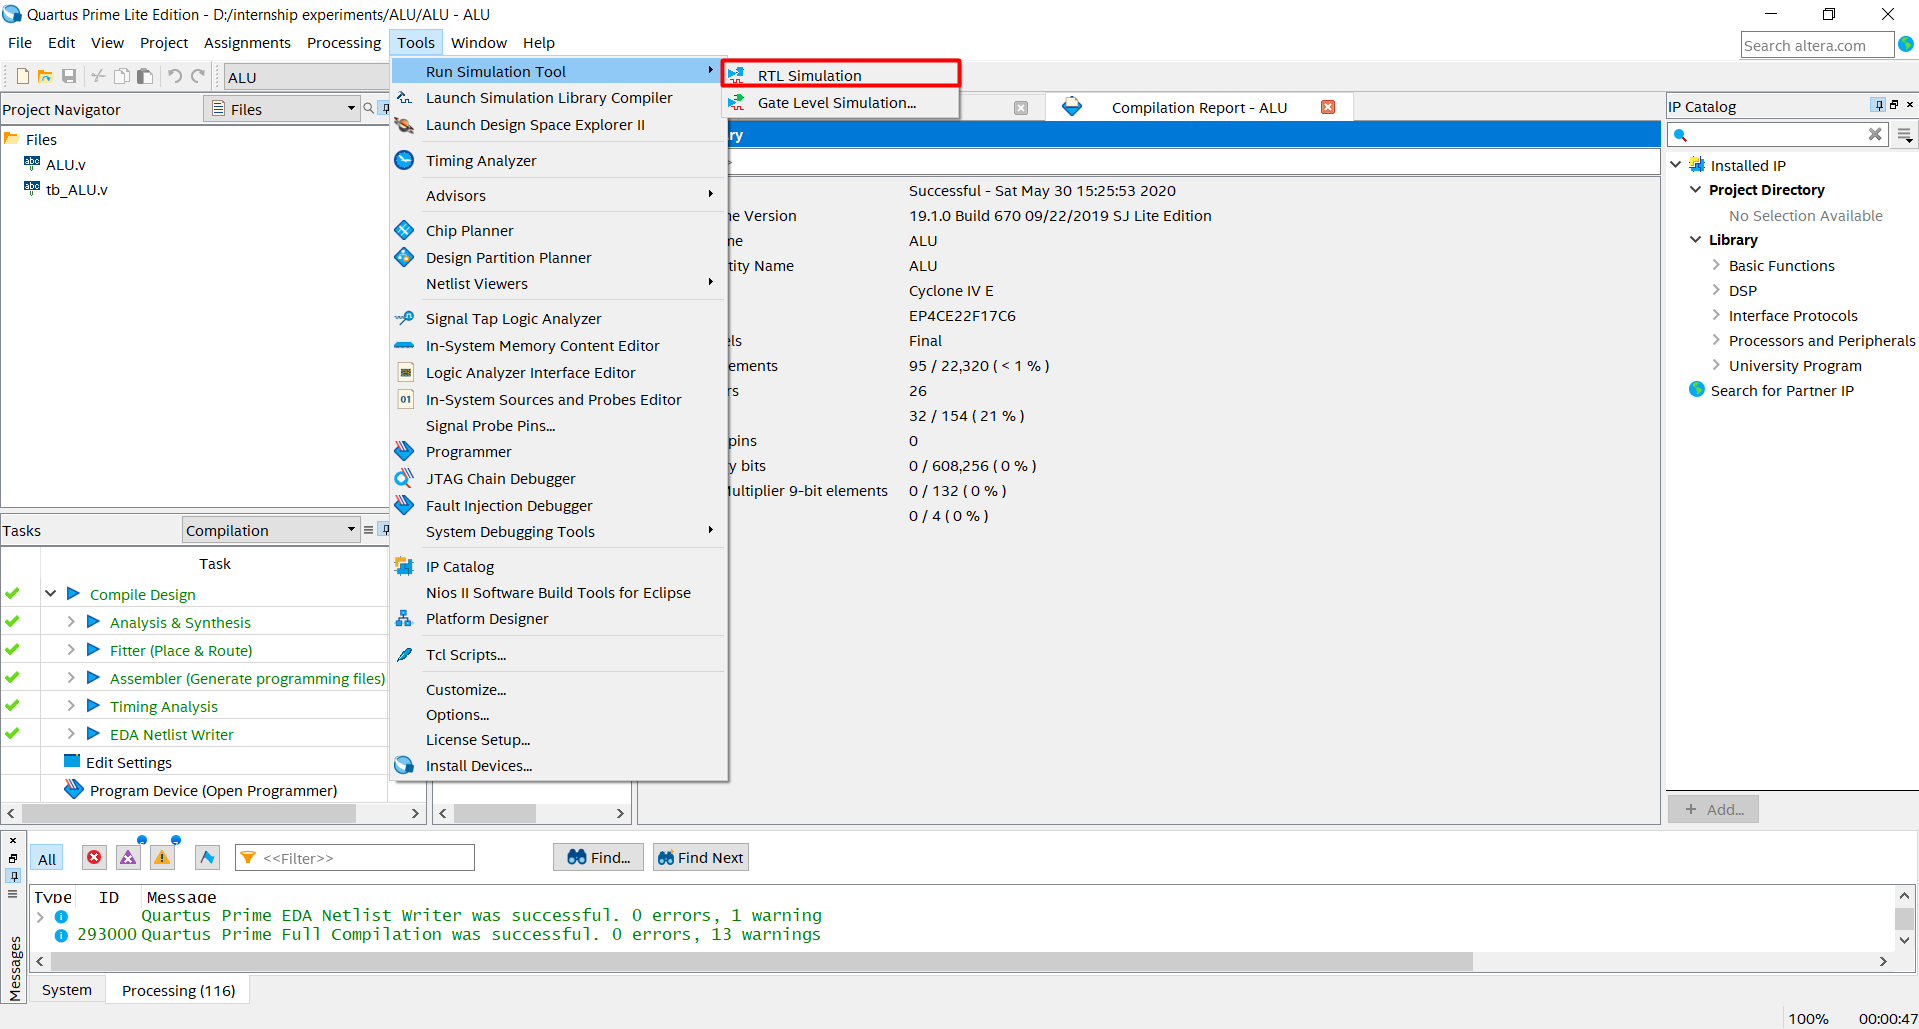
\includegraphics[width=14cm,keepaspectratio]{posttest2.png}
            \caption{RTL Simulation}
            \end{figure}

        \item Finally ModelSim-Altera tool opens up with simulated waveform. click on \textbf{Run all} icon on the tool box to display the waveform.
            \begin{figure}[H]
                \centering
                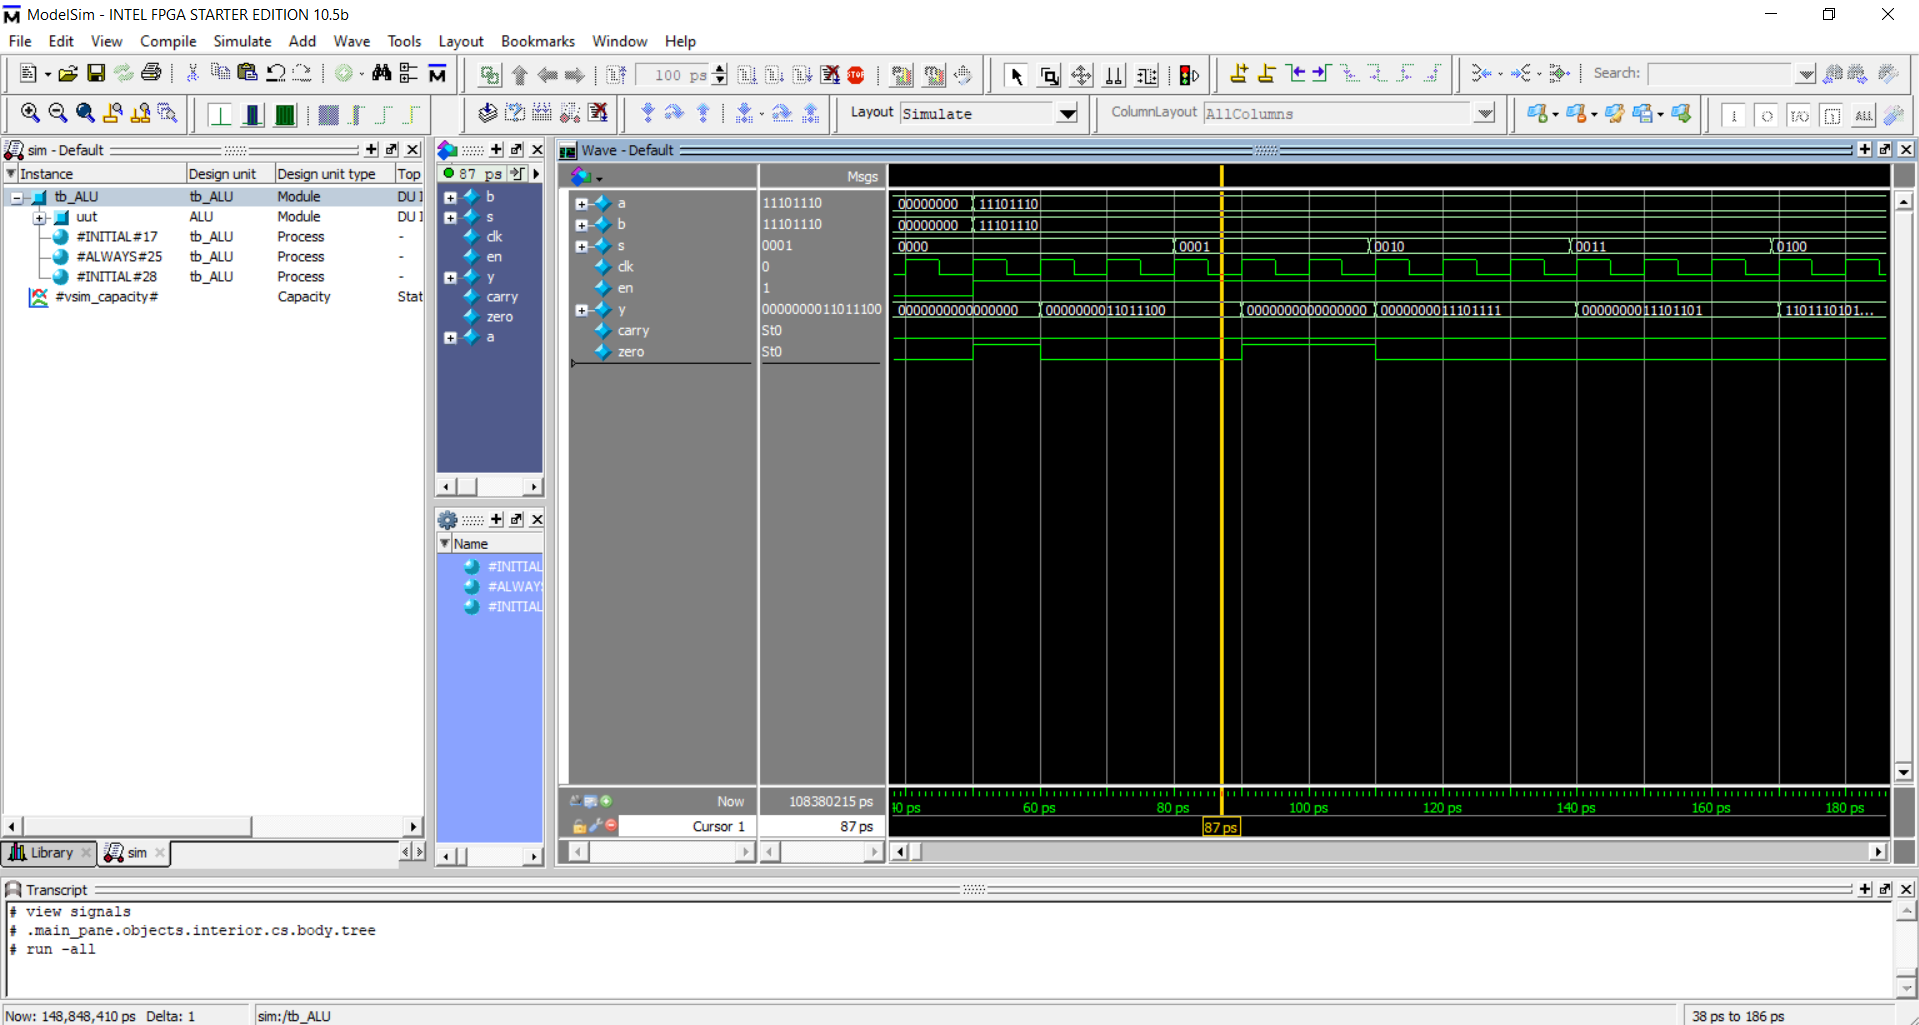
\includegraphics[width=14cm,keepaspectratio]{waveform1.png}
            \caption{RTL Simulation}
            \end{figure}
        
    \end{enumerate}
\newpage
\section{Simulation Results}

\subsection*{Simulation waveform of the Verilog Design}
The Result shown below can be verified by comparing it with the Truth Table \\provided in page 4.\newline
You can observe individual bits of a particular signal by clicking on the '+' icon.\\
\textbf{Observation:} Based on the select input\textbf{'s'} the opertion is performed on input \textbf{'a'} and \textbf{'b'} and the 16 bit result is generated on output line \textbf{'y'}.The \textbf{carry} flag is raised when carry is generated and \textbf{Zero} flag is raised if the result is zero during the operation.

\begin{figure}[H]
    \centering
    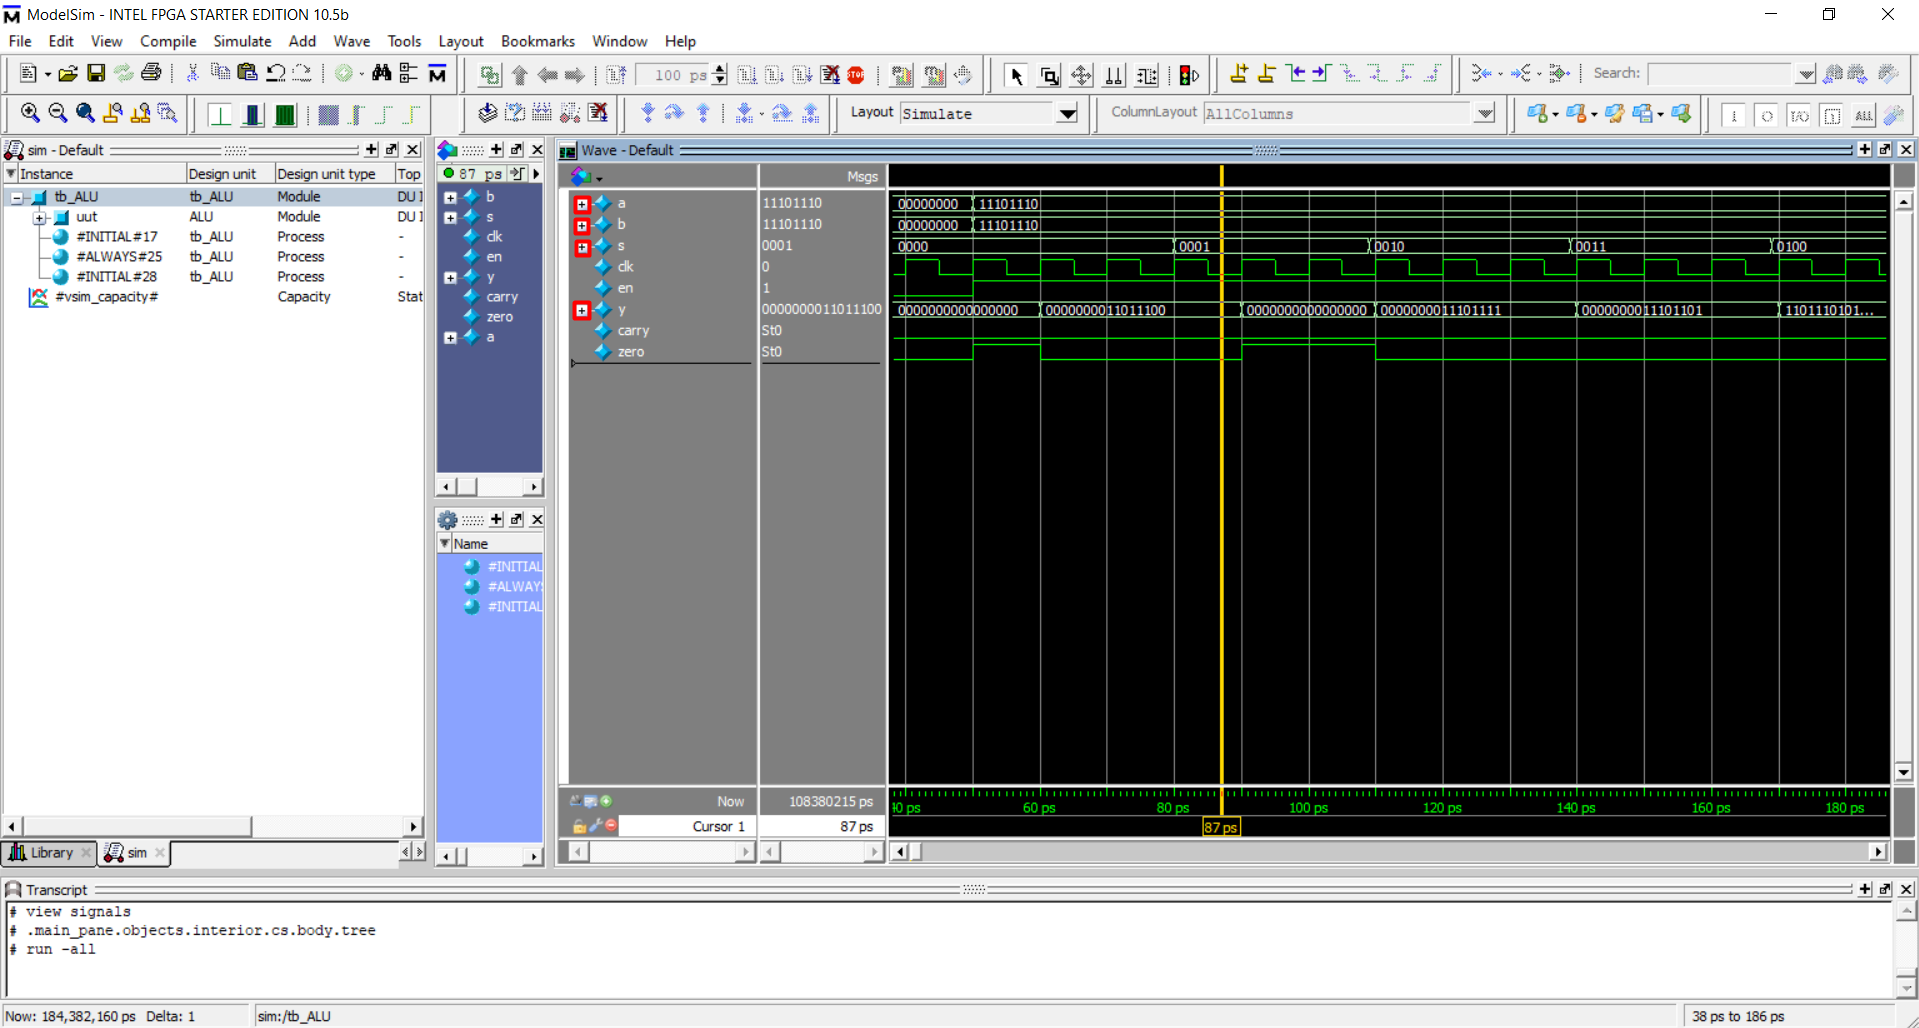
\includegraphics[width = 14cm,keepaspectratio]{waveform1n.png}
\caption{Simulation waveform}
\end{figure}

\end{document} 
 
